
\chapter{Super-resolution PSF model of HST WFC3-IR\chaplabel{wfc3ir}}

This \paper\ is joint work with Ross~Fadely (Insight) and David~W.~Hogg (NYU) and it is being prepared for submission to a refereed journal. 

\section{Chapter abstract}

Obtaining an accurate model of the Point Spread Function is crucial for reliable point source photometry, astrometry, and weak lensing studies.
The PSF model of the $\hst$ $\wfc$ IR channel does not meet the accuracy required by these science goals. 
In addition, the PSF of the $\hst$ $\wfc$ IR channel is poorly sampled. Weak lensing studies of poorly resolved images of faint distant galaxies demand 
excellent knowledge of the PSF sampled at a resolution higher than that of the $\hst$ $\wfc$ pixels.

In this \paper\, we present a generative forward model of every image taken by the $\wfc$ IR channel as a set of a number of point sources convolved
with the instrument PSF. We focus on modeling the pixel-convolved PSF, which is the optical PSF convolved with the pixel response function. 

In particular, we model the images of point sources observed in the calibration program of the $\hst$ $\wfc$ IR channel in the \emph{F160W} bandpass. 
We expect the inference of the super-resolution PSF in other filters of the IR channel to follow a similar procedure. 
We discuss how the optimal solution of the problem can be found by adopting a variance model that correctly takes into account the model 
uncertainty, a regularization term that imposes a smoothness condition on the super-resolution PSF, and masking strategy for reducing the impact of overlapping sources on 
likelihood optimization. 

\section{Introduction}

The Point Spread Function (hereafter PSF) determines the fraction of photons from a given point source that land at a particular displacement 
from the center of that point source on a detector. The PSF of the $\hst$ $\wfc$ camera is under-sampled. That is, if a center of an observed star lies 
on the center of a pixel, a significant fraction of the brightness of that star will be 
encapsulated by the single pixel that contains the centroid of the star.
In other words, within the full-width half-maximum (FWHM), the PSF is usually not spanned by multiple detector pixels since the pixels are large. 
This is mainly the result of a compromise made in design of the detectors to cover a wider field of view.

Poor sampling of the PSF by detectors renders many astronomical image processing tasks difficult. Precise astrometry and photometry 
of individual point sources requires knowledge of the PSF sampled at a higher resolution than that of the detector pixels. 
In uncalibrated observations, the images of stars are generated by convolution of the point sources with the PSF and multiplication 
with a non-uniform detector sensitivity called the \emph{flat-field}. Flat-field corrections are important for photometry and astrometry of 
individual point sources. In under-sampled images, capturing the sub-pixel variations of the flat-field requires having a high resolution 
model of the PSF. 

Furthermore, cosmic shear studies require accurate measurement of the shapes of individual distant galaxies. The galaxies used for estimation 
of the cosmic shear signal are faint and often barely resolved by the $\hst$ $\wfc$ detectors. In order to reliably measure the shapes of these poorly 
resolved galaxies, we need to convolve the model describing the light distribution of these galaxies with a higher resolution PSF model. 
Therefore, knowing the high resolution PSF is an essential ingredient in weak lensing studies of galaxies detected by the $\hst$ $\wfc$ IR 
channel.   

In this investigation, we focus on modeling the \emph{pixel-convolved PSF}, which is the optical (instrumental) PSF convolved with the 
pixel response function. It is the pixel-convolved PSF that can be directly estimated from observation without making any assumption 
about the sensitivity of detector pixels. Moreover, it is the pixel-convolved PSF that can be used to perform astrometry and photometry measurements as well as 
galaxy shape measurement for weak lensing analyses. All of these involve fitting a model to the pixel-convolved PSF. 

Another benefit of working with the pixel-convolved PSF is that the centers of pixels simply sample the PSF. That is, no integration of the 
optical PSF is required to evaluate the model of the images of point sources in observations.

Alternatively, one can deliver a model of the optical (instrumental) PSF based on physical models of the telescope optics. 
This involves measurement or prediction of the optical wavefront at all locations across the focal plane and the use of physically motivated parameters 
to model the image produced by the wavefront. Significant progress has been made in exploring the space of physical models that can reasonably 
describe the optical PSF \citep{zernike,krist1995,krist2011,galsim_software}. 

Development of optical models of the PSF are valuable efforts for simulation, validation, and understanding of the systematic uncertainties 
that can affect astronomical inferences \citep{great3,galsim}. In practice, however, using the optical PSF for photometry, astrometry and weak lensing studies 
requires fitting a star's model to the wavefront PSF model. The major drawbacks of this approach are the following: $(i)$ This approach does not make use of the available observed 
data, and $(ii)$ it makes strong assumptions about the sensitivity of detector pixels when it is used for model fitting. Therefore we attempt to build a 
data-driven or empirical model of the PSF. From now on in this \paper\, we refer to the pixel-convolved PSF as the PSF. 

This \paper\ is structured as follows: In Section~\ref{sec:hstdata} we discuss the observations and data reduction. In Section~\ref{sec:hstmethod} we discuss the algorithm we 
have developed for inferring the super-resolution PSF model of the $\hst$ $\wfc$ IR channel observations. In Section~\ref{sec:hstresults} we present the preliminary results, and %FIXME
in Section~\ref{sec:hstsummary} we summarize and conclude. 

\section{Data}\label{sec:hstdata}

The $\wfc$ IR camera takes images through four filters: F105W, F125W, F140W, F160W.
In what follows in the rest of this \paper\ we focus on modeling the images of point sources in the F160W filter of $\hst$ $\wfc$ IR channel. 
In our analysis, we make use of the FLT images that are calibrated with the recent models of charge transfer efficiency, flat-field, etc. 
We choose not to use drizzled images \citep{drizzle,astrodrizzle} because they introduce correlated noise and 
distortions to the PSF that are not consistent across the image (a new algorithm developed by \citealt{olic} for the WFIRST mission does not suffer from these issues). 
These distortions pose a challenge for optimal extraction of the PSF information and accurate measurement of shapes of galaxies. Therefore we find the pixels in the FLT images to be better-suited for PSF modeling. 

For each FLT image, we follow the following procedure to select stars with sufficiently high signal-to-noise ratio 
for PSF modeling. First the Source Extractor software \citep{sextractor} is run on each image to detect the objects. 
For each object, the stellarity index and blending/error flags are extracted. An object is called a \emph{star} if no blending/error flag is 
raised, its stellarity index is greater than 0.8, and if its peak pixel brightness value is 25 times greater than the median pixel brightness 
value.  

The FLT files obtained from the HST MAST archive \footnote{\url{https://archive.stsci.edu}} are accompanied by Data Quality extension files. 
While extracting the super-resolution PSF model from the point sources in FLT images, pixels with data quality other than zero are flagged and we do not include them in model fitting. This requirement ensures that the damaged pixels do not contribute to the PSF model. For each point source, we extract a 25 pixels $\times$ 25 pixels patch that is centered on the brightest pixel of the point source.   

\section{Method}\label{sec:hstmethod}

\subsection{generative model}

We build our empirical model of the PSF by assuming that a given point source at the center of a patch can be described by 
the following quantities: 

\begin{itemize}
\item A global solution for the super-resolution PSF $X$ that is shared between all point sources across the field of view. We assume 
that $X$ is normalized to one and it is centered at the center of the central pixel of the patch. This super-resolution PSF is sampled on 
a grid with a higher resolution than the native pixel grid of $\hst$ $\wfc$ IR observations.

\item Centroid coordinate of a point source at a given patch $\Delta_n = (\Delta x_n, \Delta y_n)$. 
These two parameters dictate the offset between the position of the centroid of the point source $n$ with 
respect to the center of the patch. Because we have centered our 25 $\times$ 25 patches on the brightest pixel, we expect these offsets to be small.

\item Flux quantity $f_n$ which is related to the brightness of the point source in each patch.

\item A background quantity $b_n$ which sets the brightness level of the background sky in each patch.

\end{itemize}

Given these ingredients, we write down the generative forward model of the point sources in the center of patches in the following way:

\begin{eqnarray} \mathbf{d}_{n} &=& \mathbf{m}_{n} + \mathrm{noise}, \label{eq:model1} \\
       m_{n,i} &=& f_{n}K^{(n)}_{il} (\Delta_n) X_{l} + b_{n}. 
\label{eq:model}
\end{eqnarray} 

In Eq.~\ref{eq:model1}, $\mathbf{d}_{n}$ is the observed 625-dimensional vector describing the brightness of the pixels in the 25 pixels $\times$ 25 pixels patch $n$. 
$\mathbf{m}_{n}$ is the model that describes the pixel-convolved model of the point source sitting on the center of the patch $n$ with the same dimensionality. The 
noise term $\mathrm{noise}$ has a variance that we present shortly.
In Eq.~\ref{eq:model}, the operator $K^{(n)}(\Delta_n)$ is a linear operator that maps the super-resolution PSF $X$ to a downsampled PSF at the native 
data grid. That is, when this operator acts on $X$, it samples $X$ on a downsampled grid (with the same resolution as the observations) 
that is shifted with respect to the grid on which $X$ is defined. The shift between the two grids is given by the vector $\Delta_n = (\Delta x_n , \Delta y_n)$.


We want to be able to explicitly construct these matrices so we can analytically compute the likelihood function and its derivative with respect to the super-resolution PSF $X$. 
We implement the linear sampling operator $K$ with bivariate cubic-spline interpolation. By comparing our implementation of cubic-spline with that of the open source 
software $\mathtt{scipy}$ we note that they have consistent performances.

It is worth noting that there exist many possibilities for designing the sampling operator $K$.  The simplest and fastest approach that one could 
choose is bilinear interpolation. But after applying this method to simulated PSFs, we find that this method lacks the accuracy we 
need. Ideally, one could use a sinc interpolation \citep{bickerton,galsim}, which is an optimal choice for preserving information.
But we find sinc interpolation to be computationally demanding. Under same assumptions, we experimented with Gaussian Process interpolation for designing the downsampling matrix $K$, but Gaussian Process interpolation requires additional computing time to set hyper parameters.


The factor by which the PSF is undersampled varies from one filter to another. Our strategy for inferring the super-resolution of the PSF model of F160W filter is as follows. 
We aim to estimate $X$ on a 75 pixels $\times$ 75 pixels grid, which is a resolution three times that of the native pixel grid of the observations.

\subsection{likelihood optimization}

Now that we have explained the quantities needed to describe the generative model of $\wfc$ IR observations, we 
present our strategy for estimating the values of the parameters of individual point sources $\{f_{n},b_{n},\Delta_{n}\}_{n=1}^{N}$ and 
the global solution of the super-resolution PSF $X$.


In order to estimate the PSF, we optimize the following likelihood function with respect to the parameters $\{f_{n},b_{n},\Delta_{n}\}_{n=1}^{N}$ and the PSF solution $X$:

\begin{eqnarray} -2 \ln L &=& -2 \sum_{n=1}^{N_{patches}} \ln L_{n} \label{eq:total} , \\
-2 \ln L_{n} &=& \sum_{i=1}^{N_{\rm pix}} \Big( \frac{\big(d_{n,i} - m_{n,i} \big)^{2}}{s^{2}_{n,i}} + \ln(2 \pi s_{n,i}^{2}) \Big) \label{eq:patch},
\end{eqnarray}

where $L_{n}$ is the likelihood of patch $n$, $L$ is the likelihood of the entire astronomical scene, $s_{n,i}$ is the $i$th component of the 625 dimensional vector $\mathbf{s}_n$, and 
$\mathbf{s}_n^{2}$ is variance of the noise model in patch $n$. The variance is composed of two terms, one arising from the Gaussian readout noise and another arising from the Poisson noise.
Therefore the total variance is given by a constant per-pixel variance of a Gaussian noise and a gain-like term that is proportional to the model $\mathbf{m}_{n}$ defined in Eqs.~\ref{eq:model1,model}:
\beq
\mathbf{s}_n^{2} = \sigma^{2} + g.\mathbf{m}_{n},
\label{eq:variance}
\eeq
where we extract Gaussian variance $\sigma^{2}=0.01$ and gain $g=0.05$ from the $\hst$ data. 

It is important to note that our forward model of the $\wfc$ IR 
observations given by Eq.~\ref{eq:model} suffers from multiple degeneracies. The first degeneracy is between 
the flux values $\{f_n\}$ and the super-resolution PSF $X$. This degeneracy will prevent us from finding a unique 
solution for $\{f_n\}$ and $X$. This degeneracy can be broken by introducing a regularization term to Eq.~\ref{eq:total} that imposes 
smoothness condition to $X$. 

We add the following term to the log-likelihood $L$
\beq
C_{\rm reg} = -2\ln L + \epsilon \sum_{j,k} \delta^{2}_{j,k},
\label{eq:reg}
\eeq
where the second term is the sum of the squared of the matrix $\delta$ whose $j,k$ components are given by the difference between the $j$th row and $k$th column of the super-resolution PSF 
and its nearest pixels. The prefactor $\epsilon$ sets the strength of the regularization term. This enforces our prior belief that the PSF should be a smoothly varying object.

The second type of degeneracy is between the centroid offsets $\{\Delta_n\}$ and the super-resolution PSF $X$. In order to lift this degeneracy, we do not add any regularization 
term. Instead, throughout the optimization procedure we enforce a set of conditions that break this degeneracy. These conditions enforce the super-resolution 
PSF to be normalized and centered around the central pixel of the higher resolution grid. 

For inference of the PSF, we follow an optimization procedure similar to the method of Expectation Maximization (EM). In the context of astronomy, EM has been employed in extreme deconvolution \citep{xd} and heteroscedastic matrix factorization \citep{hmf}. Finding the optimal solution of 
$X$ and $\{f_n , b_n , \Delta_n\}$ proceeds as follows. 

First we initialize the parameters $X$ and $\{f_n , b_n , \Delta_n\}$. We initialize the centroid offsets ${\Delta_n}$ by the matched-filter polynomial centroiding 
described in Chapter 1. In particular, we correlate a Gaussian kernel with FWHM of 2.0 pixels with the 5 $\times$ 5 central pixels of each patch before applying 
the polynomial centroiding method. The reason for why we apply the polynomial method to the central pixels of each patch is that many of the stars in our $\hst$ observations 
are in crowded fields and therefore applying the matched-filter centroiding method to the entire patch could lead to biases as a result of light contamination from overlapping 
or nearby sources. 

The initial background values $\{b_n\}$ are estimated by taking the median pixel value in each patch. For initializing the flux values $\{f_n\}$, first we subtract the initial 
estimates of background values from each patch. Afterwards, the $\{f_n\}$ values are initialized by computing the sum of the pixel values within 5$\times$5 apertures centered on 
the central pixels of the patches. The reason for limiting our initialization of the flux estimates to the 5$\times$5 apertures is to prevent contamination of fluxes from 
overlapping and nearby sources. Besides, since the PSF is poorly sampled, we expect the majority of the flux to be captured by a few pixels around the centers of the patches. 

Lastly, the super-resolution PSF $X$ is initialized in the following way. First we subtract our initial estimates of the sky background levels from the patches. Then we divide the 
pixel values of the patches by their corresponding initial flux estimates. Then we use the cubic-spline interpolation method to interpolate the rescaled patches to a high resolution 
75 $\times$ 75 grids that are shifted by $\{-\Delta_n\}$ with respect to the patch centers. Afterwards, we evaluate the mean of the interpolated rescaled patches 
to estimate the initial PSF. Furthermore, we normalize the PSF and interpolate it such that it is centered on the central pixel of the 75 $\times$ 75 high resolution grid.  

Now that we have initialized the parameters of our model, we present the EM algorithm for optimizing them. At every iteration, we follow this 
iterative scheme. In the $n$th patch, we update $b_n$ by optimizing $L_n$ while holding $\{f_n, \Delta_n, X\}$ fixed. Then 
we update $f_n$ by optimizing $L_n$ while holding $\{b_n, \Delta_n, X\}$ fixed. Then we update $\Delta_n$ by holding $\{f_n, b_n, X\}$ fixed. 
Once $\Delta_n$ is updated, we update the sampling matrix $K^{(n)}$ accordingly. 

After updating $\{b_n, f_n, \Delta_n\}$ for all patches, we update $X$ 
by optimizing the regularized cost function $C_{\rm reg}$ given in Eq.~\ref{eq:reg}. At every iteration, we normalize the super-resolution PSF and 
interpolate it such that it is centered on the center of the 75 $\times$ 75 grid. We repeat these iterations until the value of regularized cost function 
$C_{\rm reg}$ converges.

So far we have not addressed the problem of how our generative forward model of the patches takes into account the contamination arising from overlapping 
or nearby sources. In order to alleviate this issue, we introduce an additional noise model for identifying and masking out pixels that are 
in ill-fit portions of the patches.

The variance of this noise model is given by
\beq
\tilde{\mathbf{s}}_n^2 = \sigma^{2} + g\mathbf{m}_{n} + q\mathbf{m}_{n}^{2},
\label{eq:modified_variance}
\eeq 
which is similar to the variance given by Eq.~\ref{eq:variance} but with an additional term is 
proportional to the squared, downsampled model describing the patch. This accounts for possible discrepancies between the downsampled PSF model of the 
point source at the center of the patch and the observed pixels. That is, it is an effective model ``wrongness term'' term. 

This variance is used in a $\chi^2$ clipping technique to mask out ill-fit portions of the patches. 
This clipping step will prevent the the pixels affected by nearby sources to bias the inferred parameters.
In particular, after every model realization we identify the pixels that are not faithfully represented by the model and mask them so they do not 
contribute to computation of the patch likelihood function (\ref{eq:patch}).
 
At every iteration of optimizing the patch log-likelihood function, we mask out the pixels for which a clipped $\chi^{2}$ 
(denoted by $\chi^{2}_{clip}$ from now on) is larger than 3. For a given patch $n$, the clipped $\chi^{2}$ is defined in the following way:
\beq
\chi^{2}_{n,\mathrm{clip}} = \frac{(\mathbf{d}_{n} - \mathbf{m}_{n})^{2}}{\tilde{\mathbf{s}}_{n}^{2}}, 
\label{eq:chi_clip}
\eeq
where $\tilde{\mathbf{s}}_{n}^{2}$ is given by Eq.~\ref{eq:modified_variance}. In a given patch $n$, the log-likelihood pixels with $\chi^{2}_{n,\mathrm{clip}} > 3$ 
do not contribute to computation of $L_n$ and its derivatives with respect to model variables. 
We set the parameter $q$ to 1. We note that this choice of does a good job at masking out the pixels that receive light from the nearby or overlapping sources. 
In principle $q$ needs to decrease iteratively as our knowledge of the PSF improves. In this work however, we choose to hold the value of $q$ fixed at one. 


%\begin{algorithm} 
%\caption{The procedure for Inferring the Super-Resolution PSF}
%\begin{algorithmic}[1] \label{alg:supermean}

%\IF{$t=1:$}
%\STATE $\epsilon_t \gets \infty$
%\FOR{$n=1,...,N$}
%   \STATE // \emph{This can now be done in parallel for all i}
%
%   \STATE $b_{n}$ \gets \mathrm{median} \; $(y_{n})$
%   \STATE $f_{n}$ \gets $\sum_{i=1}^{N_pix} \big(y_{n,i} - b_{n}\big)$
%   \STATE \mathrm{Initialize} $\Delta_{n}$ with the 3 \times 3 polynomial method
%   \STATE $X_{n}$ \gets \mathrm{cubic \; spline} $(\Delta_n)[\big(y_{n,i} - b_{n}\big)/f_n]$
%\ENDFOR
%\STATE $X$ \gets $\sum_{n=1}^{N} X_{n]$%

%\ENDIF
%\IF{$t=2,...,N_{it}:$}
%\FOR{$i=1,...,N$}

%   \WHILE{$\rho(X,D)>\epsilon_t$}
%   \STATE Draw $\pars^{*}_{t}$ from $\{\pars_{t-1}\}$ with probabilities $\{w_{t-1}\}$
%   \STATE $\pars^{*}_{t} \gets K(\pars^{*}_{t},.)$
%   \STATE $X = f(\pars^{*}_{t})$
%   \ENDWHILE
%   \STATE $\pars^{(i)}_{t} \gets \pars^{*}_{t}$
%   \STATE $w^{(i)}_{t} \gets \pi(\pars^{(i)}_{t}) / \big(\sum\limits_{j=1}^{N}w_{t-1}^{(i)}K(\pars^{(j)}_{t-1},\pars^{(i)}_{t}) \big)$
%\ENDFOR
%\ENDIF

%\end{algorithmic}
%\end{algorithm}

\section{Preliminary Results}\label{sec:hstresults}

With the ingredients of our methodology explained in Section~\ref{sec:hstmethod}, we now present the results of applying our 
method to the observations of the point sources in the $\hst$ $\wfc$ IR channel. We train our PSF model with a number of 
patches that were selected such that majority of them only contain one point source. 

In principle given the methodology explained in Section~\ref{sec:hstmethod}, we can train our forward model on patches with arbitrary 
number of stars. But in order to minimize the training time as much as possible, we select a set of isolated and 
relatively high signal-to-noise ratio stars as our training sample.
It is important to note that selecting patches containing isolated sources does not necessarily guarantee that there is \emph{no} light contamination 
by the nearby sources. %Even in the absence of additional sources in a given patch, there could be some light contamination by bright objects in nearby patches.

Therefore it is necessary to follow the procedure explained in the previous section to clip the pixels that may have received light 
contamination from the nearby sources. The parameter $q$ will be held at the constant value of $q=1$ and any pixel with $\chi^{2}_{\rm clip} > 3 $ 
will not be permitted to contribute to the likelihood function. 
This will ensure that the ill-fit portions of the training pixels will not bias the final PSF estimate. 

Note that we also need to set the strength of the smoothness regularization term $\epsilon$. Here, we can take advantage of the patches that were not used 
in training the PSF model to perform cross-validation. Cross-validation can be done in the following way. A set of values $S_{\epsilon}$ for the parameter $\epsilon$ need to be selected. For every $\epsilon$ in $S_{\epsilon}$, the optimization procedure as described above can be followed to to estimate $X_{\epsilon}$ which is the estimated $X$ corresponding to $\epsilon$. 

Then one can optimize the patch negative log-likelihood $-2\ln L_n$ given in Eq.~\ref{eq:patch} to find a solution for $\{f_n,b_n,\Delta_n\}$
variables for every patch in the cross-validation set. Afterwards, the optimal values of $-2\ln L_n$ in cross-validation patches can be summed up to 
compute the cross-validation score $C_{\rm cv}$ as a function of the regularization strength $\epsilon$.
In the end, the PSF solution $X_{\epsilon}$ that minimizes this cross-validation cost function will be selected as the optimal solution.

Although it is important to set the value of $\epsilon$ by minimizing a cross-validation score, in practice one can choose a 
value for $\epsilon$ by ensuring that neither the negative log-likelihood nor the regularization term will dominate each other. 

Choosing an arbitrarily large value of $\epsilon$ will drive the optimization procedure to only optimize the smoothness term, while choosing a very small 
value of $\epsilon$ will make the smoothness regularization negligible. We found that with $\epsilon = 1000$, the contributions received from the two terms 
of the right hand sides of Eq.~(\ref{eq:reg}) remain similar. Therefore in what follows in the remainder of this \paper\ we set $\epsilon$  to 1000.
Furthermore, we only use the validation set (patches not used in estimating the PSF) for validating our PSF model and verifying our 
methodology for masking the contribution of nearby stellar sources to patch fitting.  

In Figure~\ref{fig:srpsf} we show our initialization of the super-resolution PSF method and our final estimate of the PSF found by
minimizing Eq.~(\ref{eq:reg}). We note that in comparison to the final estimate of the PSF, our initial estimate based on scaling, shifting, 
upsampling and averaging is very smooth. Additionally, the initial PSF misses many of the sharp features and structures that exist in the optimized solution, specially along the tails of the PSF.

Performance of the method at modeling the patches in the training sample is demonstrated in Figures~\ref{fig:training_1},~\ref{fig:training_2},~\ref{fig:training_3},~\ref{fig:training_4}. 
Note that, we have \emph{intentionally} selected isolated sources with relatively high signal-to-noise ratios for training our algorithm. In addition to the data and the scaled realization of the model at the native pixel grid, we show a $\chi$ map (a measure for the goodness-of-fit), and a map of various pixels across the patch that have been flagged by the observations or the model. Pixels with $\mathtt{FLAG}=0$ are the pixels used in PSF modeling. $\mathtt{FLAG}=1$ corresponds to pixels that where flagged in MAST data quality extensions. Finally, $\mathtt{FLAG}=2$ corresponds to the group of pixels for which $\chi^{2}_{\rm clip}>3$. 

Figures~\ref{fig:training_1} and~\ref{fig:training_2} show examples of two relatively bright sources. Note that even in our training pixels, there are pixels that are ill-fit and are masked out according to the clipping criteria. Figures~\ref{fig:training_3},~\ref{fig:training_4} show the performance of our method at modeling the relatively low signal-to-noise ratio point sources in the training sample. We note that overall, the model shows a good performance at modeling these sources.

The validation set consists of stellar sources that are mostly present in crowded fields. Majority of the patches in the validation set have either more than 
one point source, or have light contamination by nearby sources. We have not used these sources in our PSF modeling but we show how our super-resolution PSF estimate 
can be used in modeling the crowded astronomical scenes in the validation set. In each patch, we optimize the patch negative log-likelihood function given in Eq.~\ref{eq:patch} to 
estimate the background sky, flux, and the centroid of the point source on the center of the patch. 

Furthermore, we use the clipping criterion $\chi^{2}_{\rm clip}>3$ to mask out pixels for which the squared model residuals are larger than modified variance (\ref{eq:modified_variance}).
Note that the masking procedure needs to be repeated at every realization of the patch model given in equation (\ref{eq:model}). After applying this clipping method to the validation set, we also decided to extend it in the following way: after every model realization and identifying the flagged pixels with $\chi^{2}_{\rm clip}>3$, we grow the flagged regions 
in every direction by one pixel. We found this to be a more conservative choice and also better at capturing the pixels that receive light from the outer tails of the PSF from other stars. In what follows, we show examples for both the original and the extended versions of our masking algorithm.

Examples of the performance of our model with a less conservative masking algorithm are shown in Figures~\ref{fig:validation_1},~\ref{fig:validation_2},~\ref{fig:validation_3},~\ref{fig:validation_4}. As it can be seen in Figs.~\ref{fig:validation_1},~\ref{fig:validation_2},~\ref{fig:validation_3}, the masking algorithm identifies majority of the pixels that are ill-fit with the PSF model (\ref{eq:model}) and prevents them from contributing to the $\chi$ map. However, there are still pixels that receive a small fraction of their brightness from the nearby point sources and are not masked out of the $\chi$ map. 

Figure~\ref{fig:validation_4} demonstrates the most extreme case in which a tail of the PSF from a very bright nearby source is present in the patch and it is not completely masked out by the original clipping algorithm. This shows the need to adopt the more 
conservative choice described above and grow the masked regions in every direction by one pixel.
Figures~\ref{fig:validation_5},~\ref{fig:validation_6},~\ref{fig:validation_7} demonstrate patch-fitting examples in which a more conservative masking algorithm is adopted. Note that in these patches most of the light received from the nearby sources or the ill-fit pixels are almost completely removed from the $\chi$ map.

\section{Summary and Discussion}\label{sec:hstsummary}

In this work, we have presented the first generative forward model of the observations of every point sources in the rich $\hst$ $\wfc$ IR dataset. 
The point spread functions of $\wfc$ IR channels are the most undersampled amongst all $\hst$ channels. 
The exercise of making highly accurate measurements of the shapes of faint and poorly resolved galaxies, accurate and precise astrometry and photometry of point sources, 
correction of the variable sub-pixel response function ``flat-field'' of the telescope, and many other scientific applications require great knowledge of 
the PSF at a resolution higher than what is sampled by the $\wfc$ IR detectors. 

Our approach differs from the analysis developed for the \emph{Euclid satellite} presented in \citet{ngole,ngole2} in that it does not attempt to infer the super-resolution PSF in a wavelet basis and it does not imposes any sparsity regularization. It assumes a more general noise model that includes both the Gaussian pixel noise and the Poisson noise arising from the instrument gain.

Our analysis is different than the approach of \citet{anderson2000} as we estimate the PSF by optimizing a well-motivated objective function 
that is based on a generative forward model of the observations. However, they are similar in that they both require regularization of the PSF model after every iteration so that the degeneracy between the super-resolution PSF and the centroids of stars can be lifted. 
The method presented in \citet{anderson2000} is based on shifting, averaging and eventually smoothing the PSF that does not involve optimizing any likelihood function.

Furthermore, it is restricted to using only the isolated point sources and it is not prone to patches in which there is light contamination by the nearby sources. 
The method presented in this \paper\ implements a rigorous treatment of every pixel that is ill-fit by the PSF model as a result of overlapping sources or light contamination by nearby sources. We implemented this by introducing a clipped $\chi^{2}_{\rm clip}$ that takes into account the model uncertainty. At every model realization throughout patch-fitting, pixels with $\chi^{2}_{\rm clip}$ more than a certain level are prevented from contributing to the likelihood function.

PSF estimation and accurate point source photometry on a crowded field has two main challenges. \emph{First}: a large fraction of the pixels may not be usable for modeling purposes. This could lead to  significant information loss. \emph{Second}: using pixels that receive photons from multiple sources in modeling the PSF can bias the final PSF estimate. 
Using a validation set containing many point sources in the crowded fields, we show that we can successfully use our technique to perform PSF-fitting. 
This allows us to make optimal use of all the pixels in $\wfc$ IR observations of crowded fields.

\section*{Acknowledgments}

We are grateful to Jay~Anderson, Dan~Foreman-Mackey, Michael~Blanton, and Alex~Malz, and Michael~Blanton for discussions related to this work.

%%%%%%%%%%%%%%%%%%%% FIGURES %%%%%%%%%%%%%%%%%%

%%%%%%%%%%%%%%%%%%%%%%%%%%%%%%%%%%%%%%%%%%%%%%%%%%%%%%%%
% PSF INITIAL AND FINAL
%%%%%%%%%%%%%%%%%%%%%%%%%%%%%%%%%%%%%%%%%%%%%%%%%%%%%%%%

\begin{figure*}
 \begin{tabular}{cc}
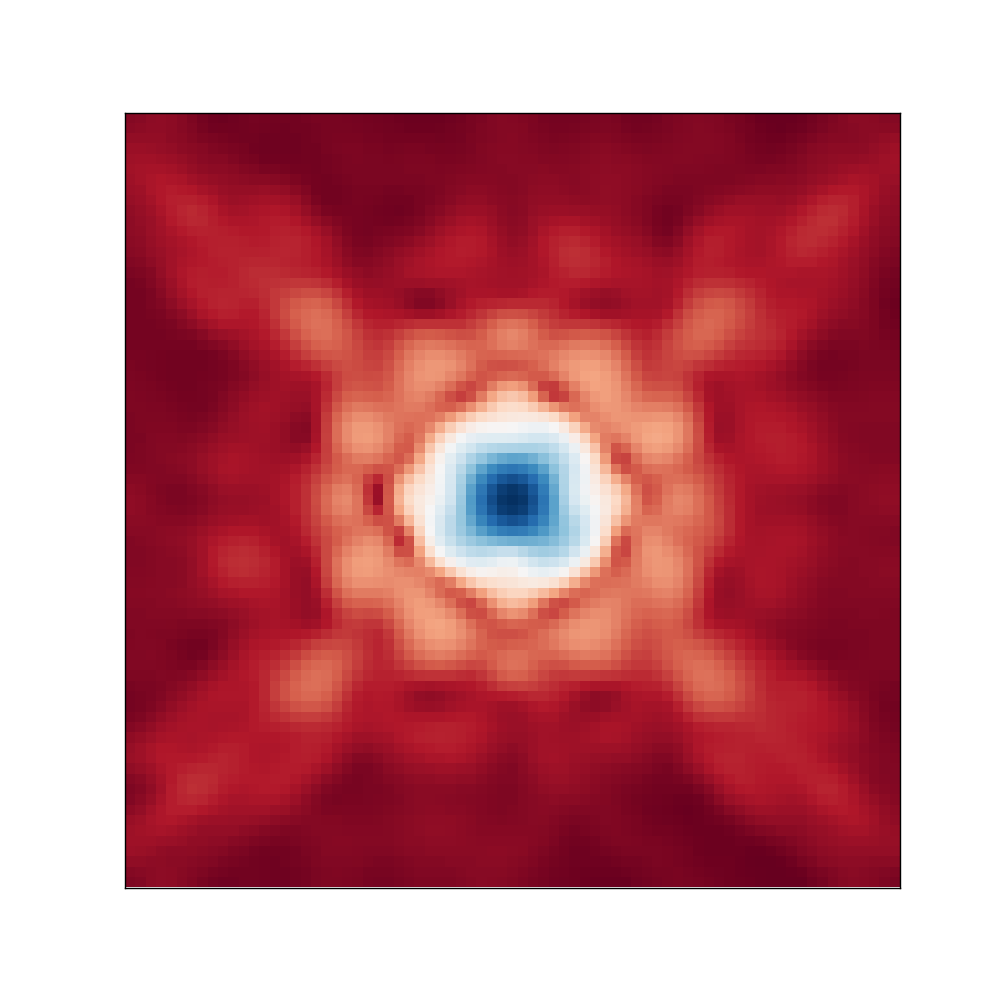
\includegraphics[width=0.5\textwidth]{figures/wfc3ir/super0.png}
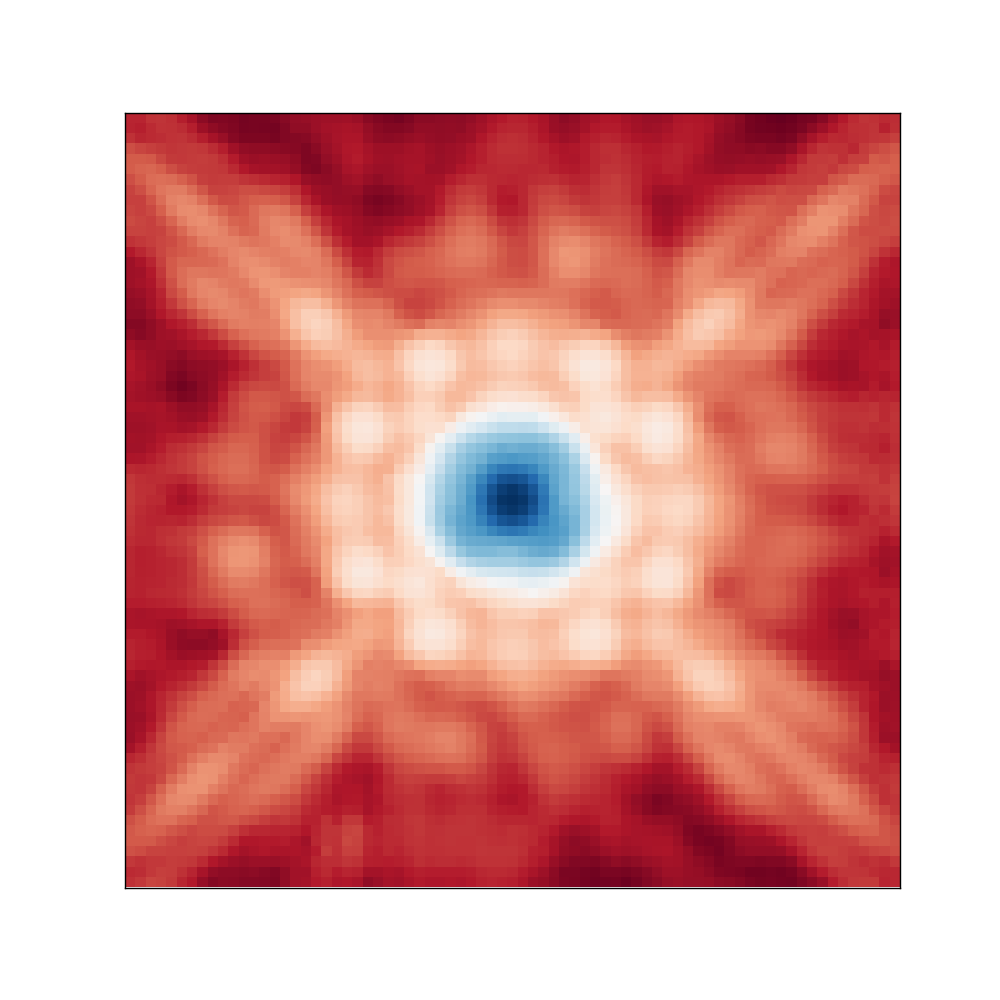
\includegraphics[width=0.5\textwidth]{figures/wfc3ir/super2.png}
\end{tabular}
\caption{\label{fig:srpsf} Left: Demonstration of the initialization of the super-resolution PSF model. The initial PSF was constructed by scaling (background subtraction and flux normalization), shifting (through matched-filter polynomial centroiding), upsampling (with cubic spline interpolation), and averaging the isolated stars in the observation sample. 
Right: Super-resolution PSF estimated by optimizing the likelihood function after six iterations. We note that the averaged upsampled initial PSF is smooth and lacks the sharp features visible across the full radian support of the PSF, specially the tails.}
\end{figure*}

\begin{figure*}
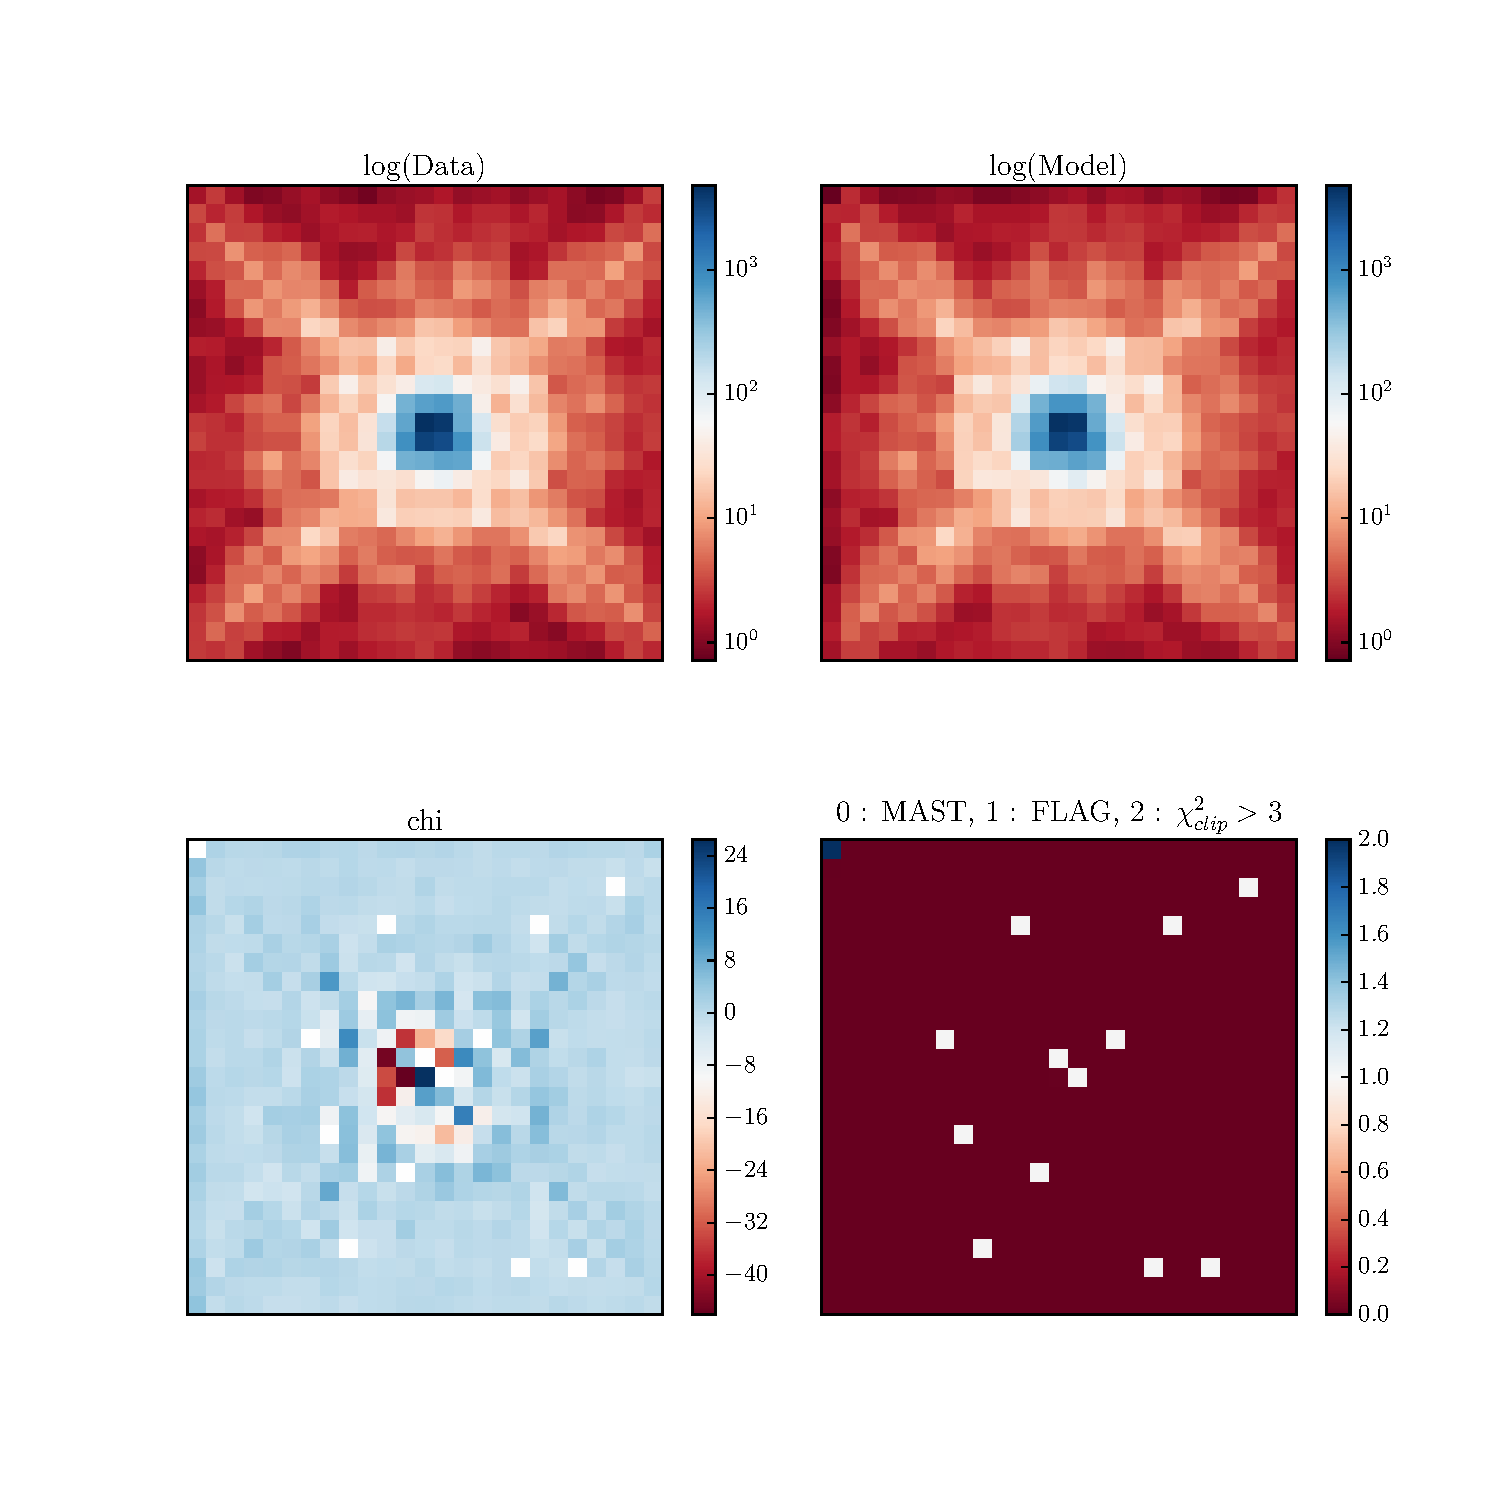
\includegraphics[width=0.9\textwidth , height=0.9\textwidth ]{figures/wfc3ir/training.pdf}
\caption{\label{fig:training_1} An example of a patch containing a high signal-to-noise ratio star in the training set. Upper-left and upper-right panels show the data and the model respectively. The lower left panel shows $\chi$. The lower right panel shows the flagged pixels. Pixels with $\mathtt{FLAG}=0$ are used in PSF-fitting. Pixels with are $\mathtt{FLAG}=1$ (provided by the MAST data) are masked out prior to the analysis. Finally, pixels with $\mathtt{FLAG}=2$ correspond to the pixels in a given model realization with $\chi^{2}_{\rm clip} > 3$.}
\end{figure*}

\begin{figure*}
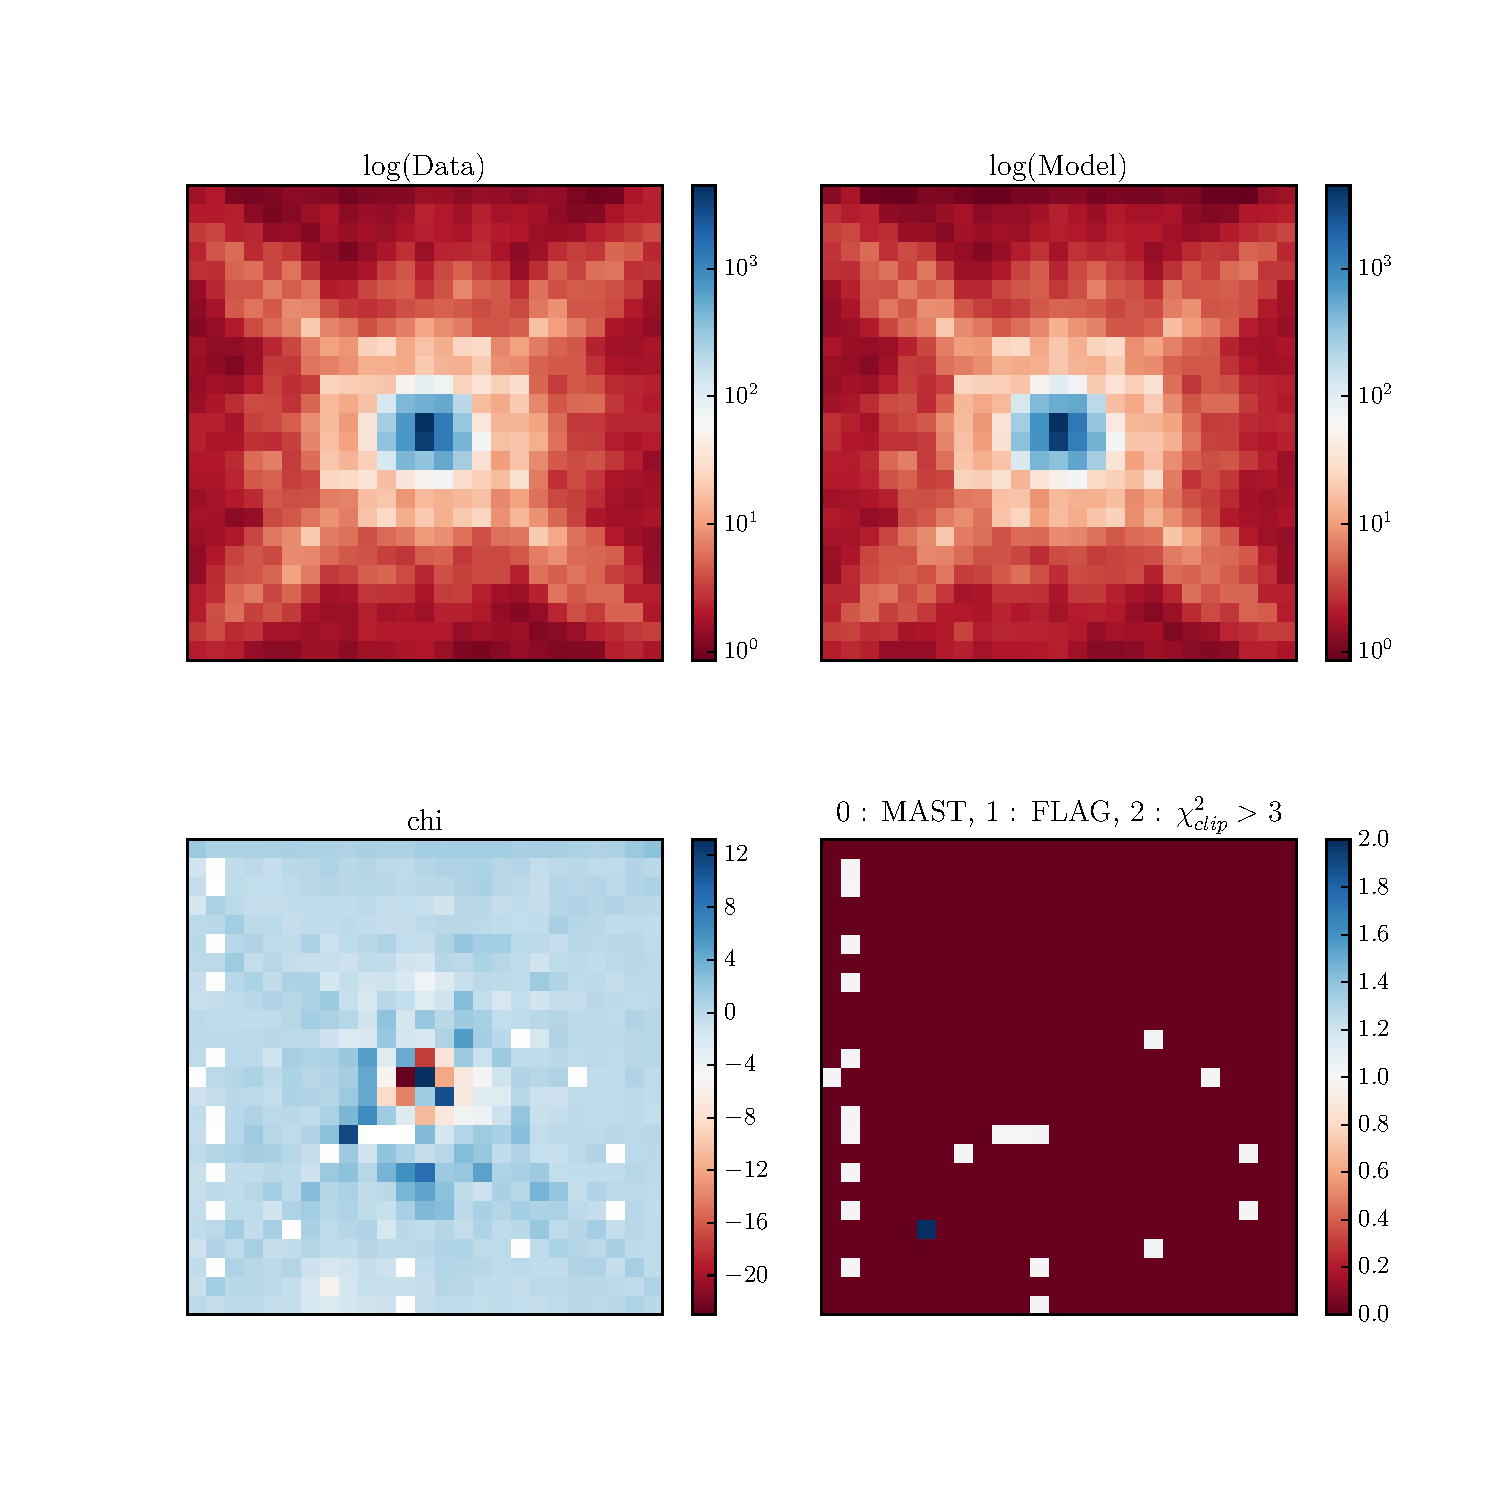
\includegraphics[width=0.9\textwidth , height=0.9\textwidth ]{figures/wfc3ir/training2.pdf}
\caption{\label{fig:training_2} Same as Figure~\ref{fig:training_1} but showing a different high signal-to-noise ratio star in the training set.}
\end{figure*}

\begin{figure*}
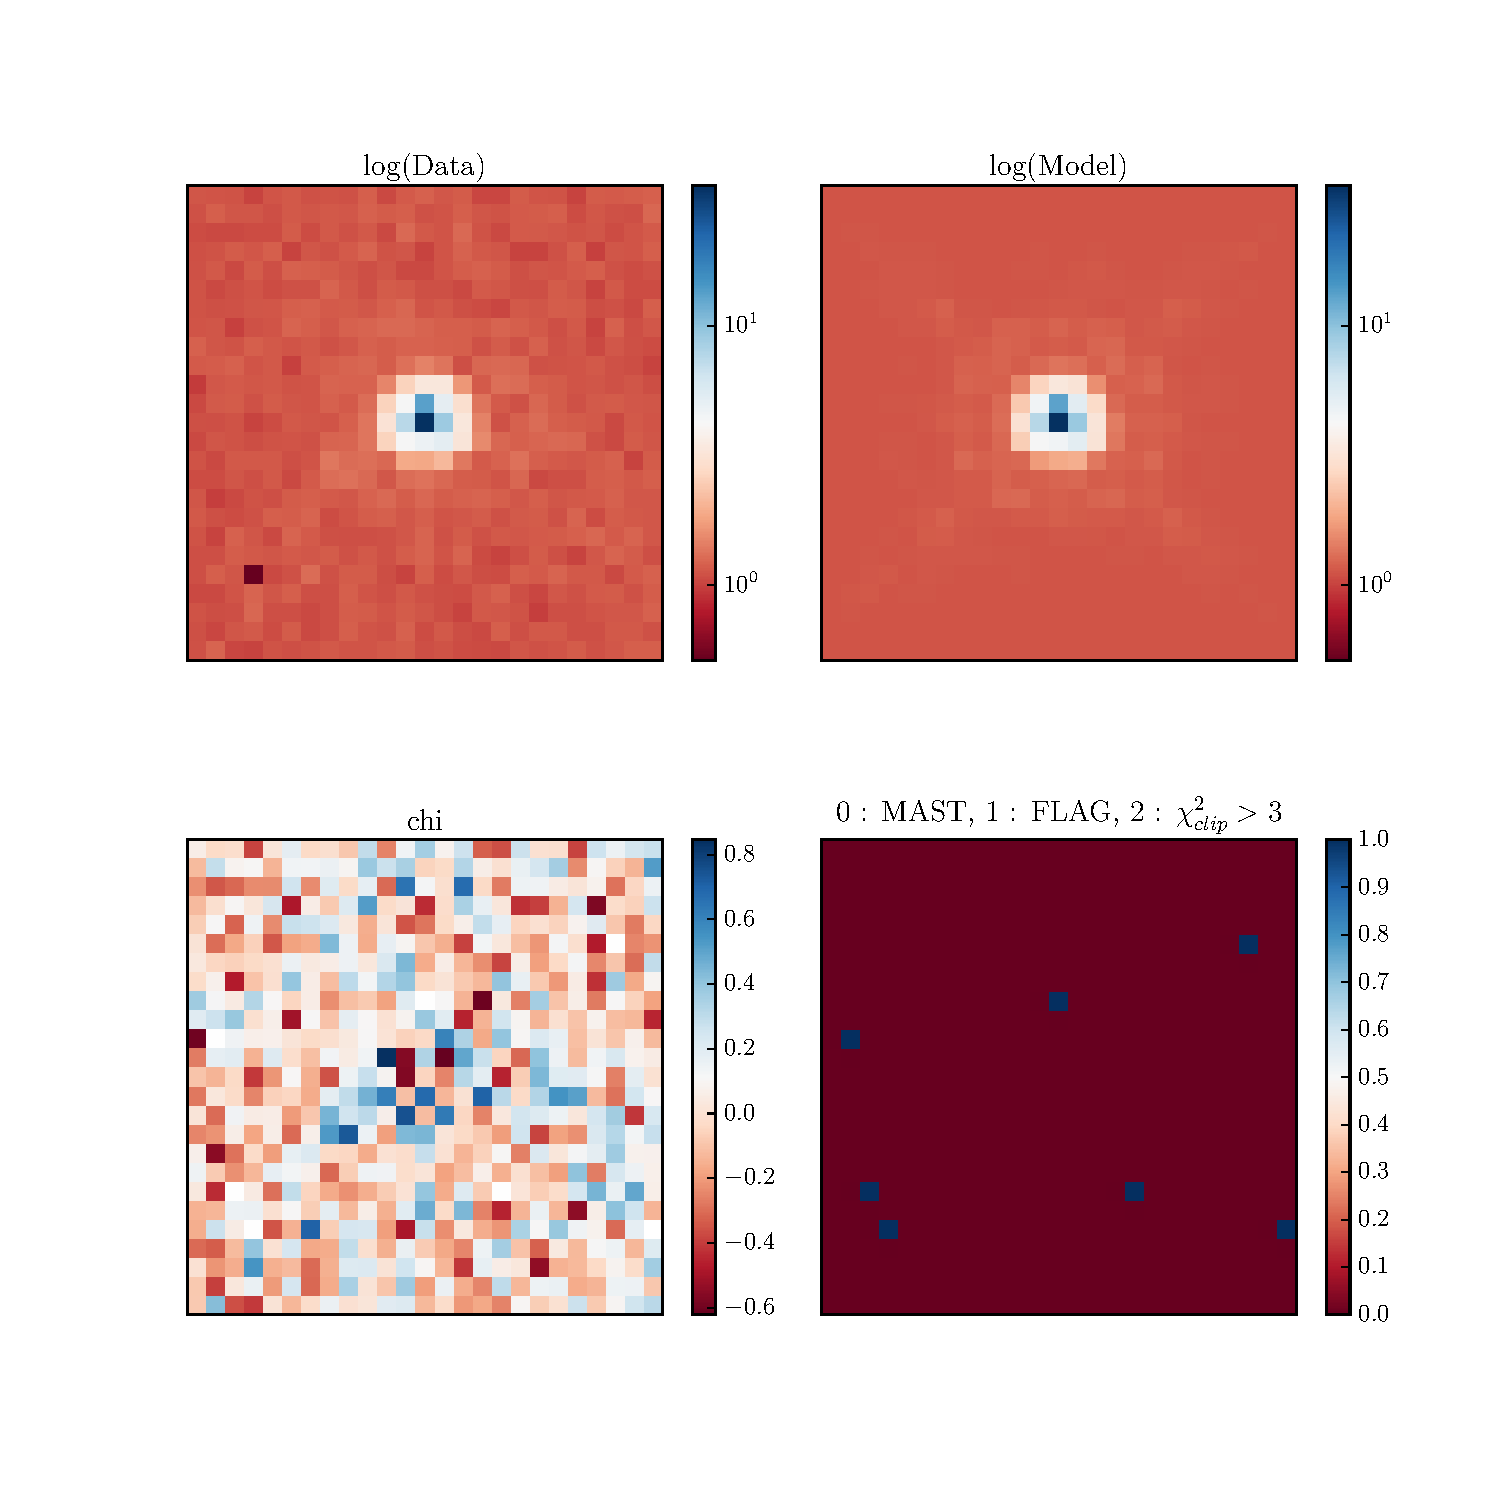
\includegraphics[width=0.9\textwidth , height=0.9\textwidth ]{figures/wfc3ir/training3.pdf}
\caption{\label{fig:training_3} Same as Figure~\ref{fig:training_1} but showing a low signal-to-noise ratio star in the training set.}
\end{figure*}

\begin{figure*}
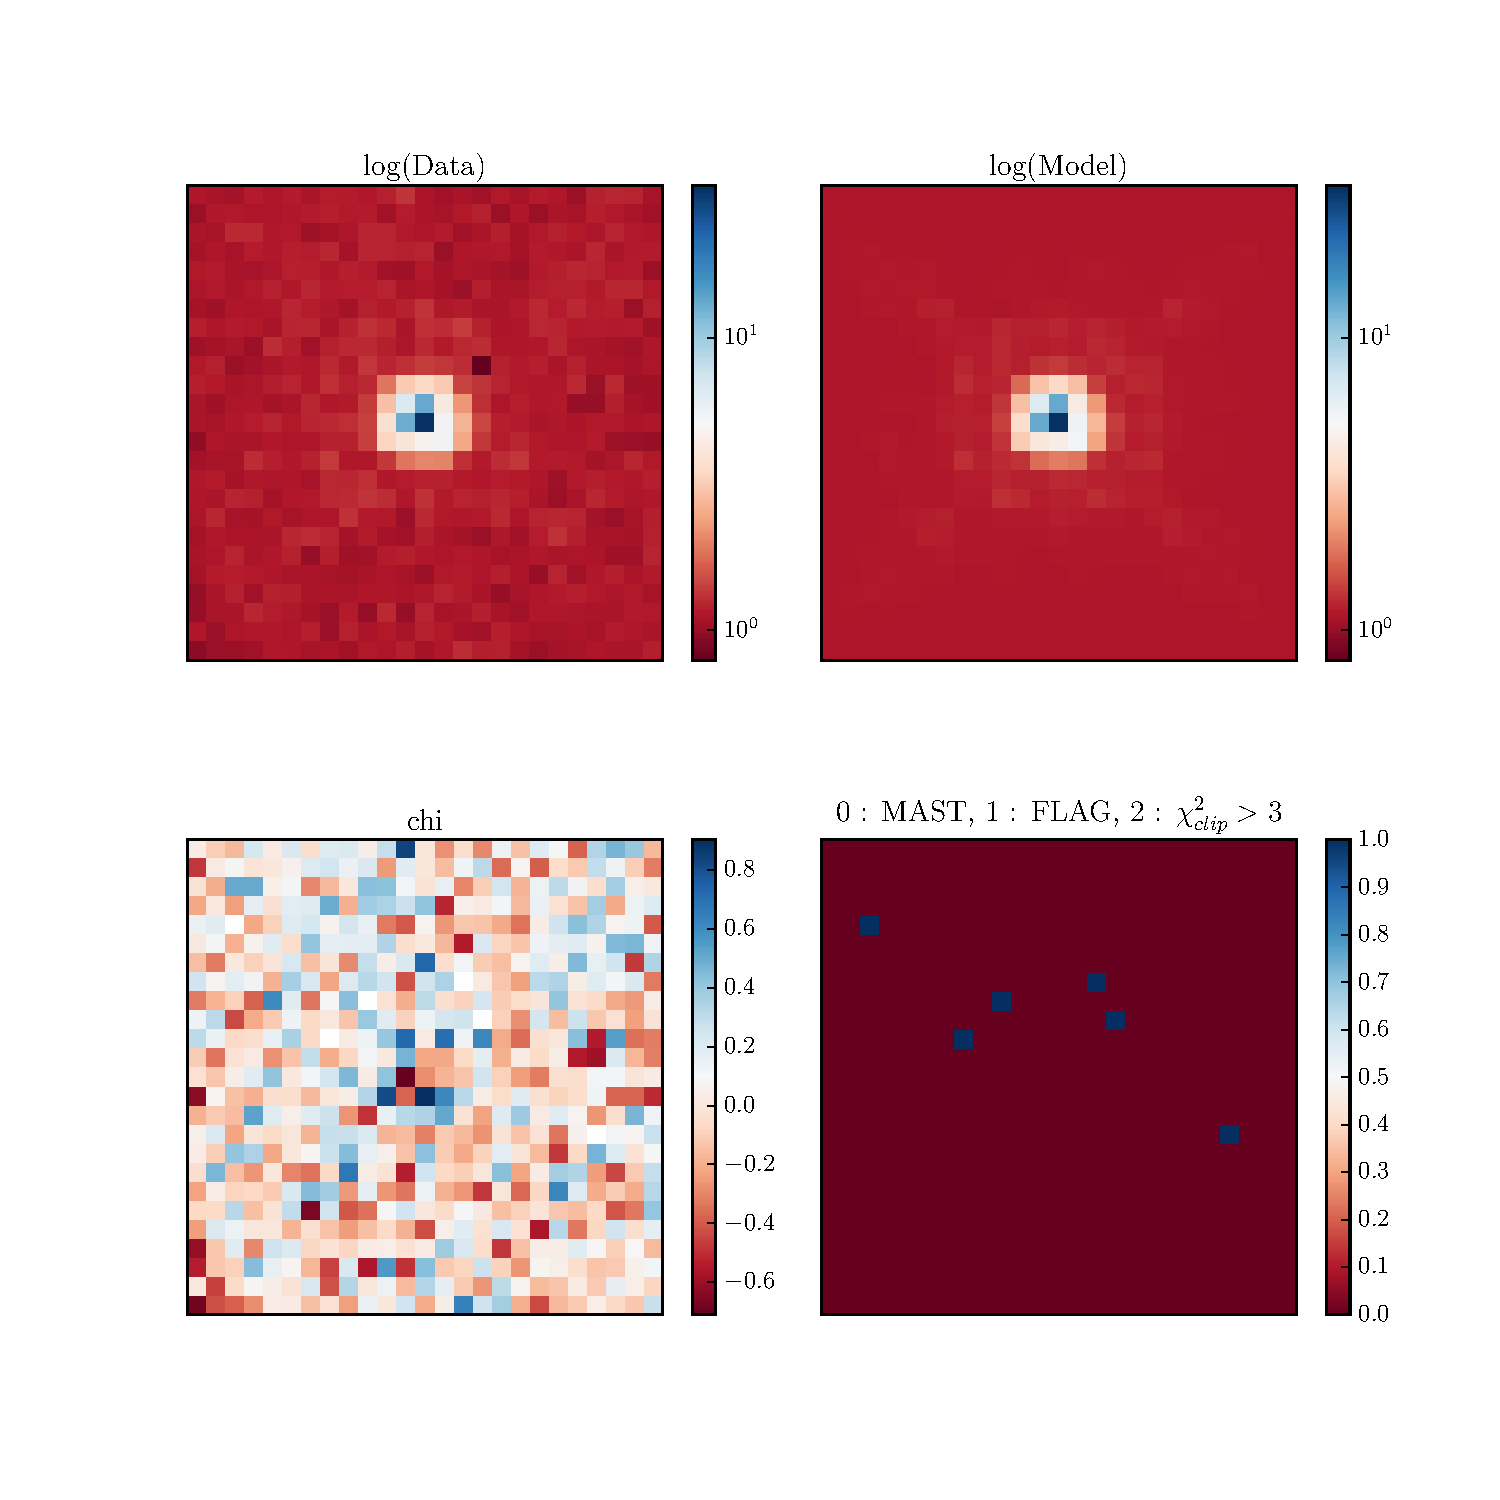
\includegraphics[width=0.9\textwidth , height=0.9\textwidth ]{figures/wfc3ir/training4.pdf}
\caption{\label{fig:training_4} Same as Figure~\ref{fig:training_1} but showing a different low signal-to-noise ratio star in the training set.}
\end{figure*}

%\begin{figure*}
%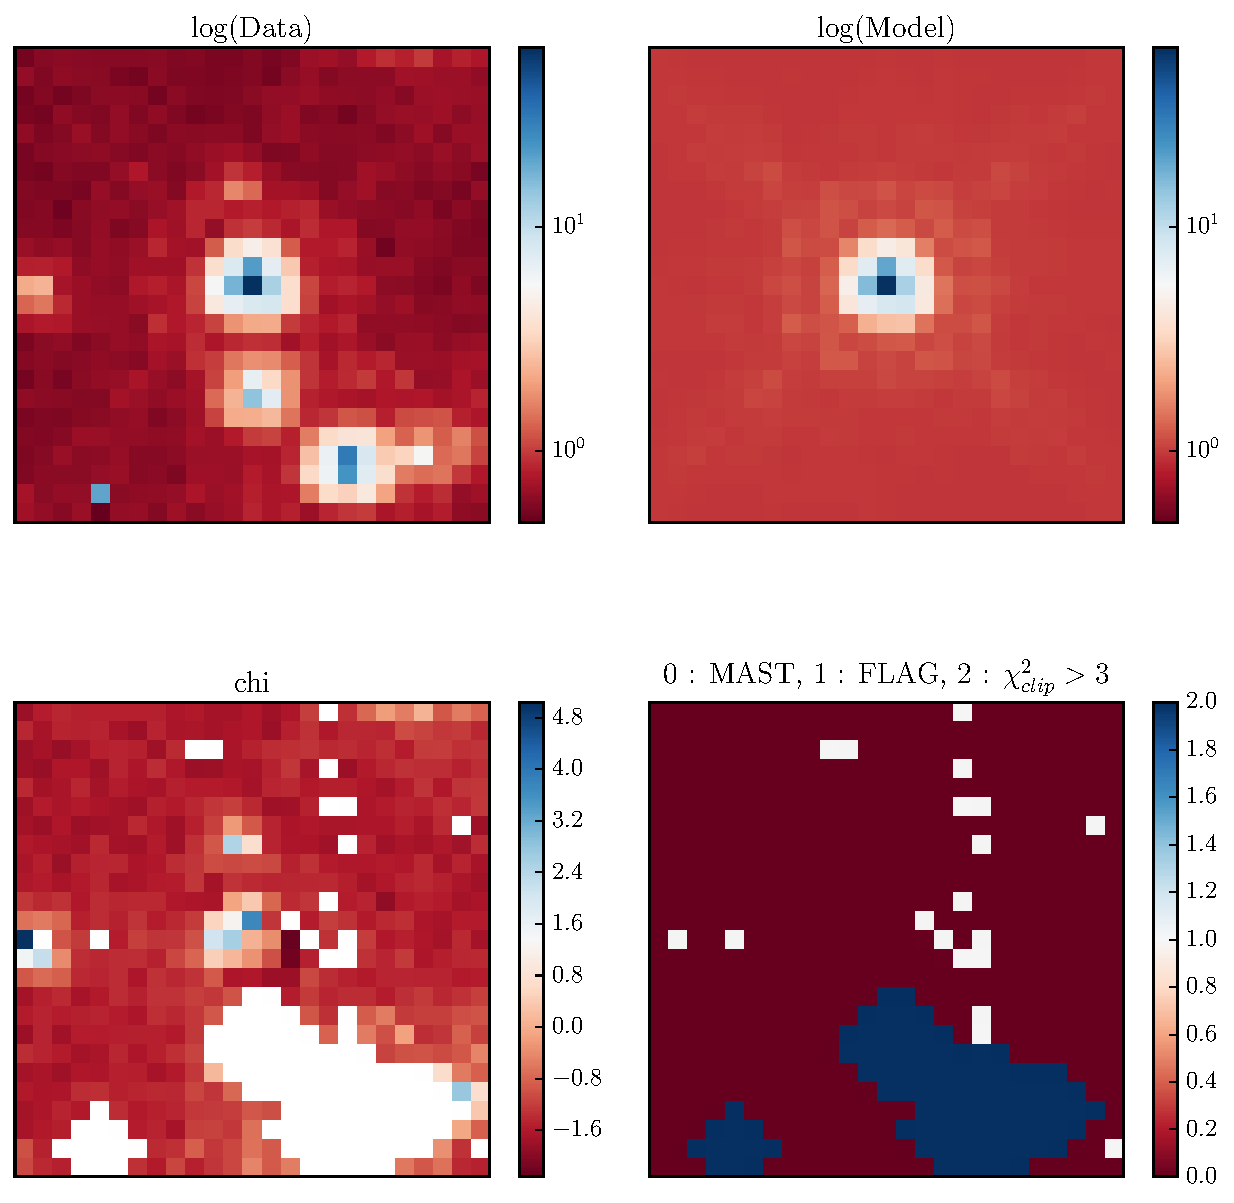
\includegraphics[width=0.9\textwidth , height=0.9\textwidth ]{figures/wfc3ir/example1762.pdf}
%\caption{\label{fig:validation_1} }
%\end{figure*}

\begin{figure*}
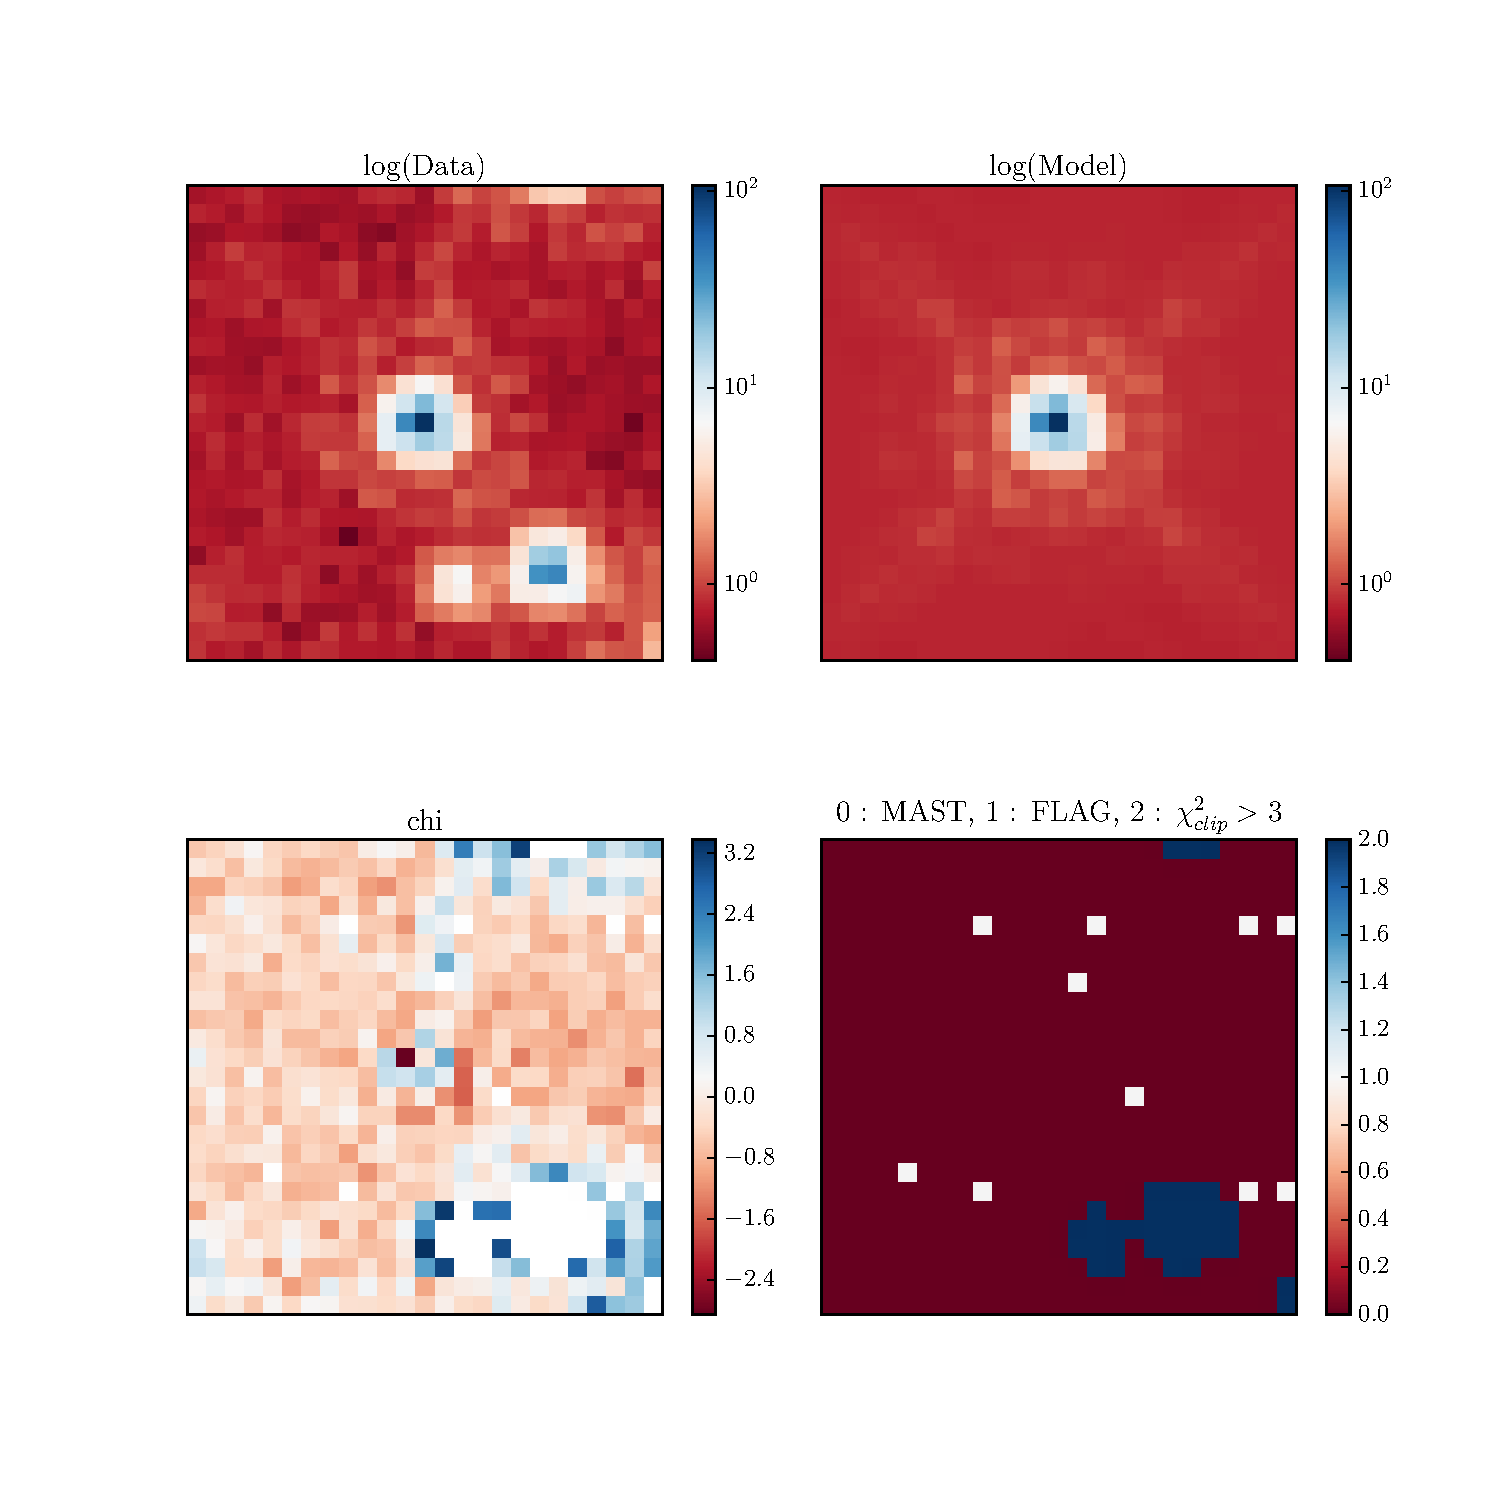
\includegraphics[width=0.9\textwidth , height=0.9\textwidth ]{figures/wfc3ir/example2.pdf}
\caption{\label{fig:validation_1} An example of a patch in the validation set containing multiple point sources. Upper-left and upper-right panels show the data and the model respectively. The lower left panel shows the $\chi$ map. The lower right panel shows the flagged pixels. Pixels with $\mathtt{FLAG}=0$ are used in PSF-fitting. Pixels with $\mathtt{FLAG}=1$ (provided by the MAST data) are masked out prior to the analysis. Finally, pixels with $\mathtt{FLAG}=2$ correspond to the pixels in a given model realization with $\chi^{2}_{\rm clip} > 3$. In the lower left panel, pixels with  $\chi^{2}_{\rm clip} > 3$ are masked out from the $\chi$ map. Note that the point sources visible in the lower right and upper right corner of the data are masked out in the $\chi$ map. Here we do not grow the masked regions and therefore a small fraction of the light from the other point sources still contribute to the map.}
\end{figure*}

\begin{figure*}
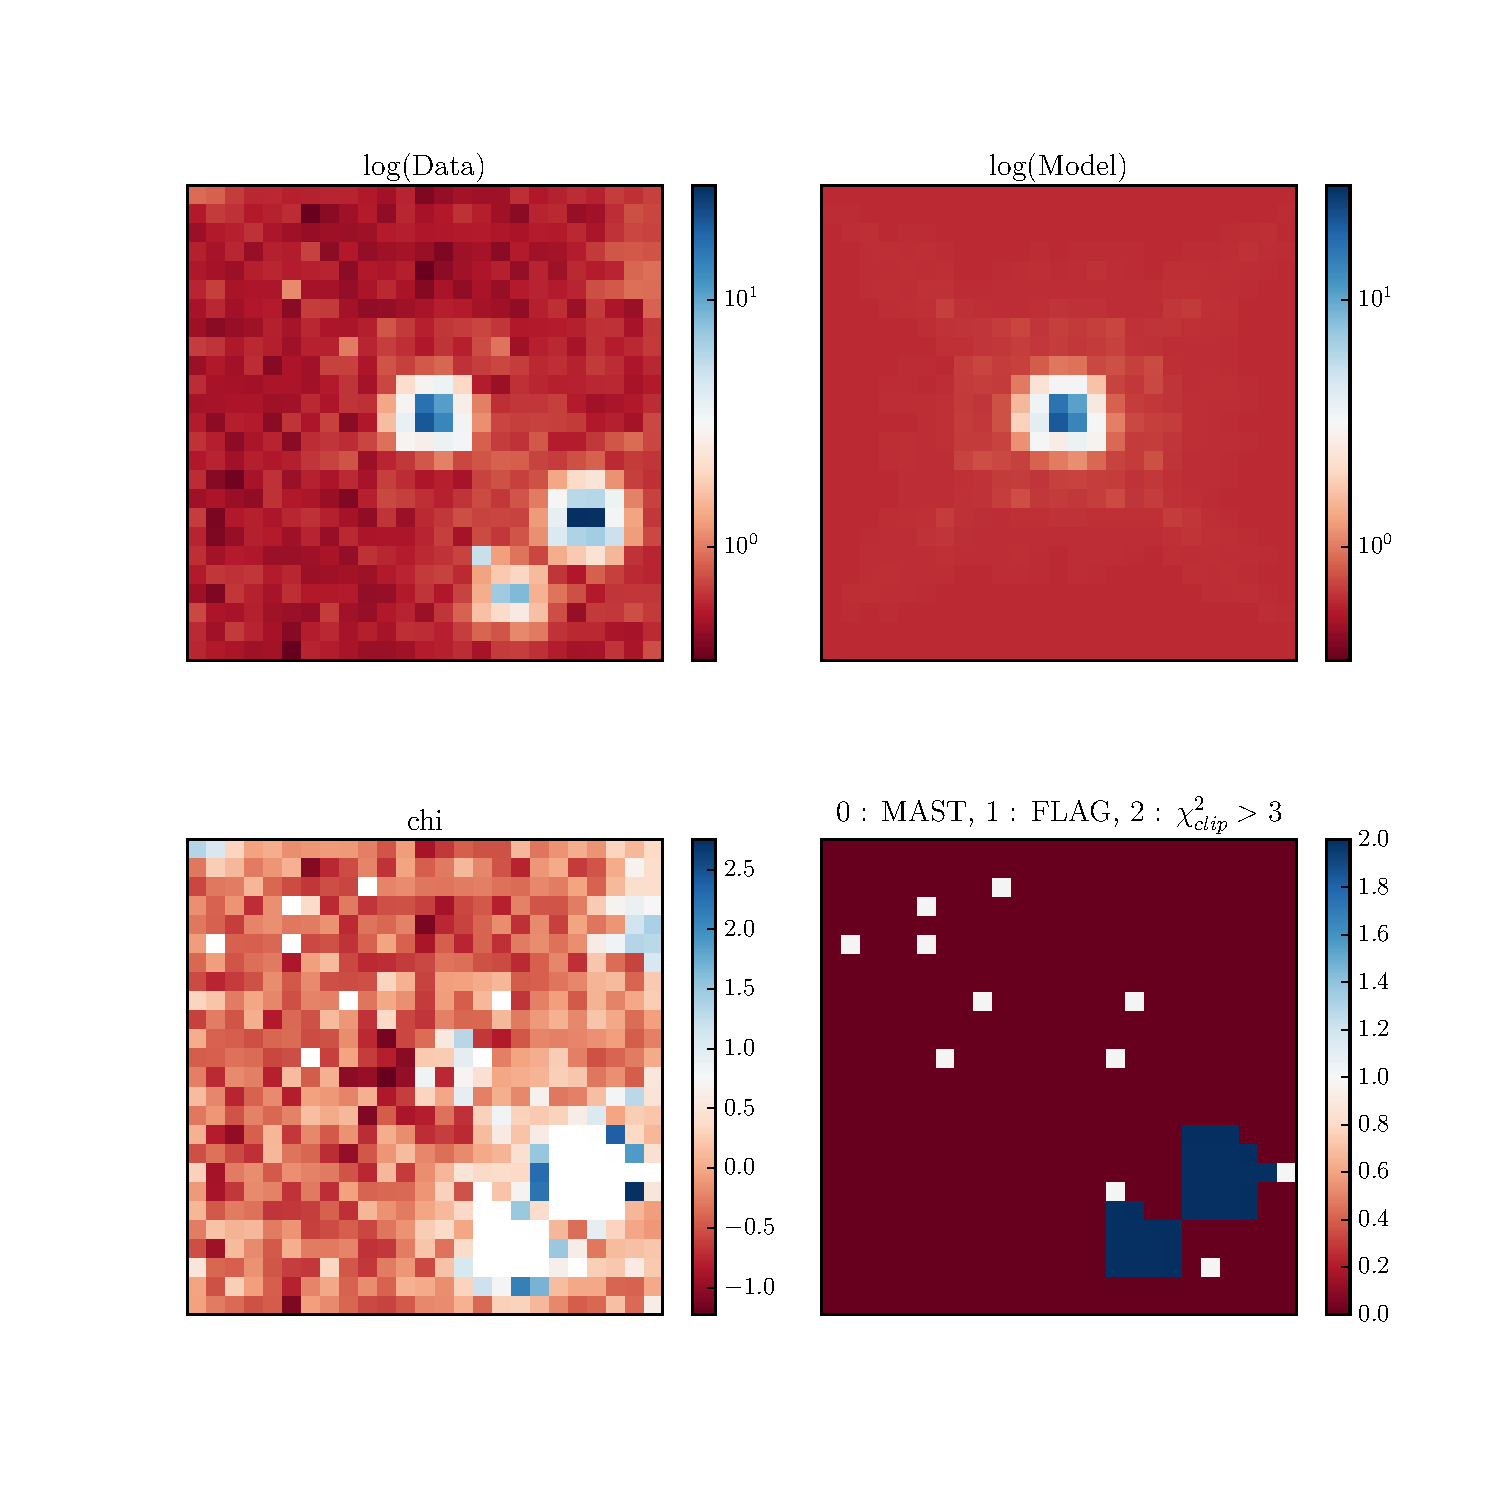
\includegraphics[width=0.9\textwidth , height=0.9\textwidth ]{figures/wfc3ir/example5.pdf}
\caption{\label{fig:validation_2} Same as Figure~\ref{fig:validation_1} but showing a different patch of sky.}
\end{figure*}

\begin{figure*}
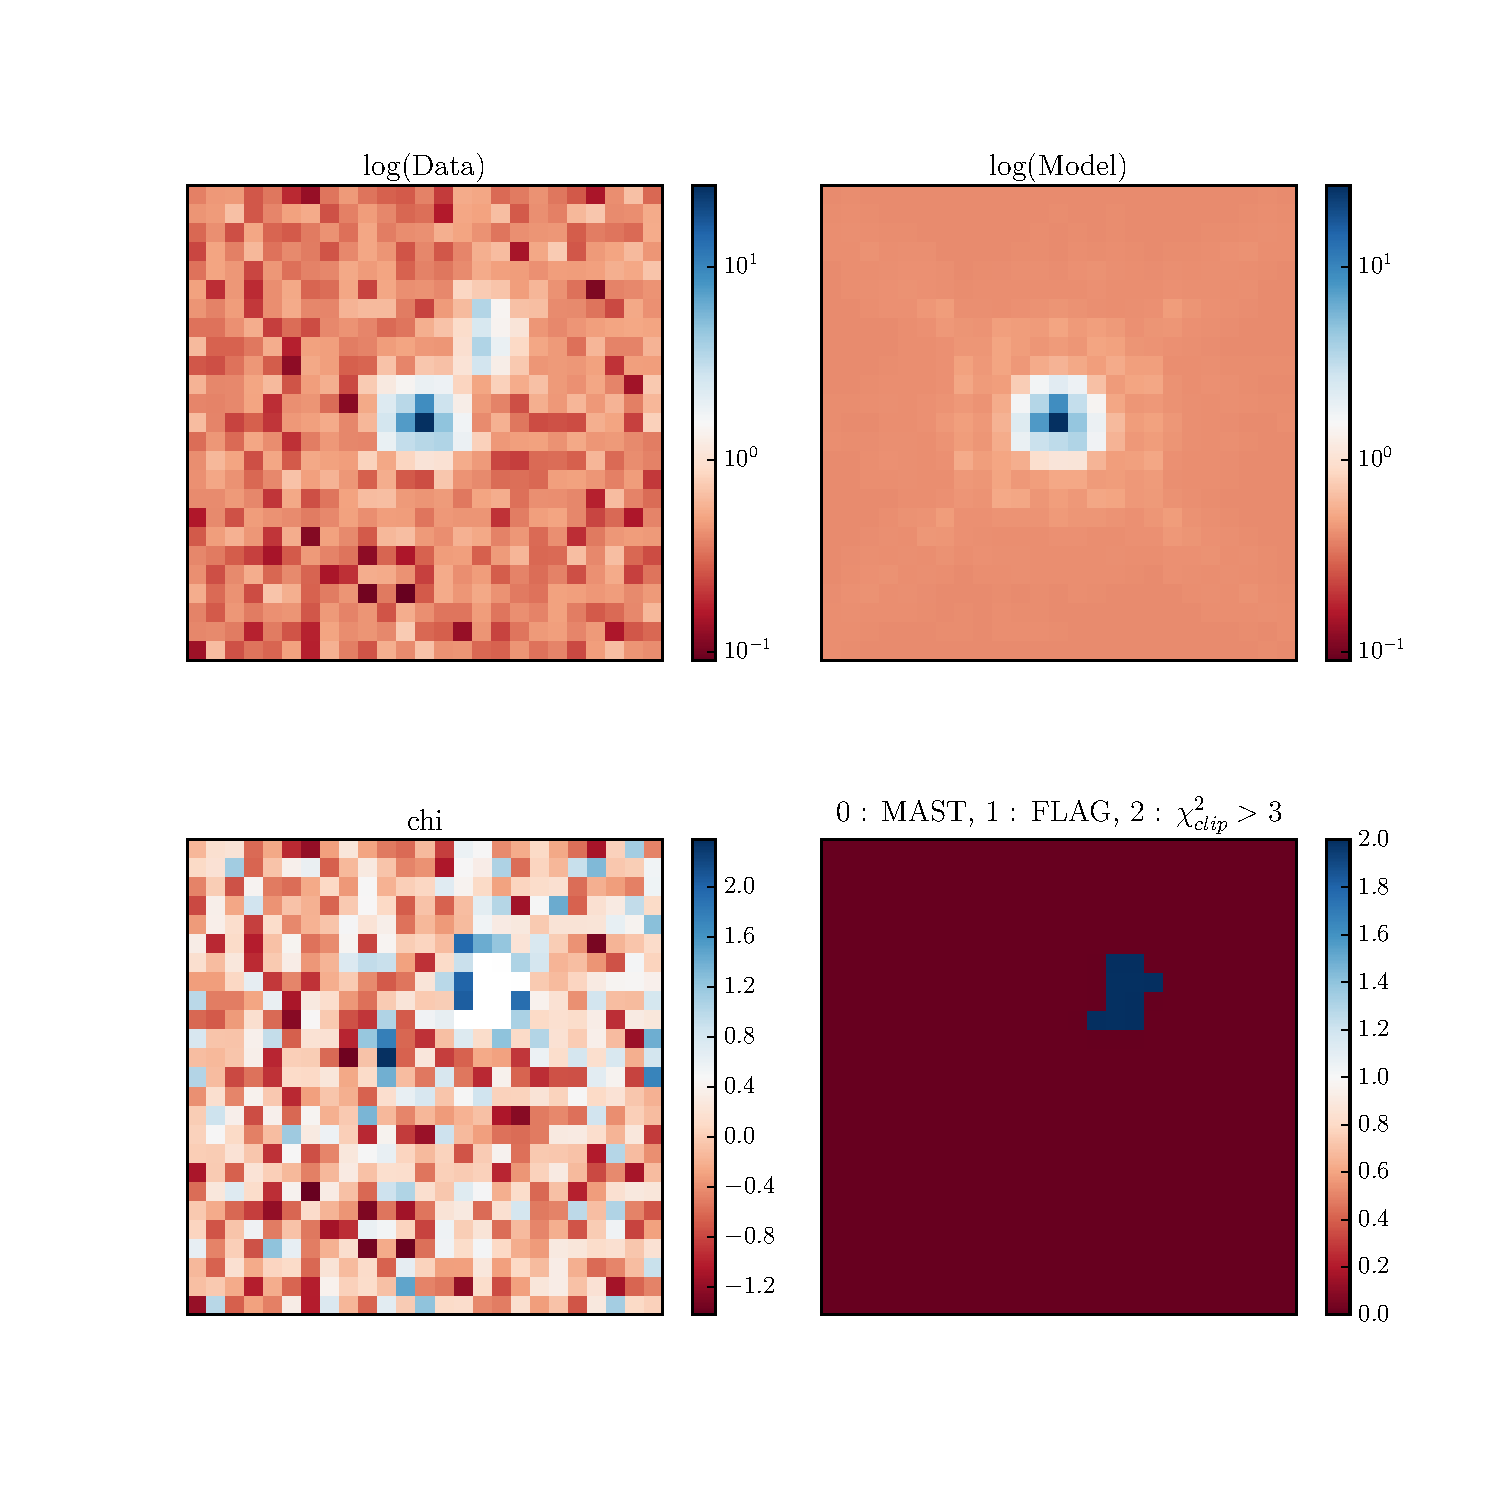
\includegraphics[width=0.9\textwidth]{figures/wfc3ir/example7.pdf}
\caption{\label{fig:validation_3} Same as Figure~\ref{fig:validation_1} but showing a different patch of sky. Two nearly overlapping faint point sources are present in this patch. 
The clipping algorithm masks out the second star. Since we do not grow the masking regions in this example, it is likely that the second faint star could still have slight contribution to the $\chi$ map.}
\end{figure*}

\begin{figure*}
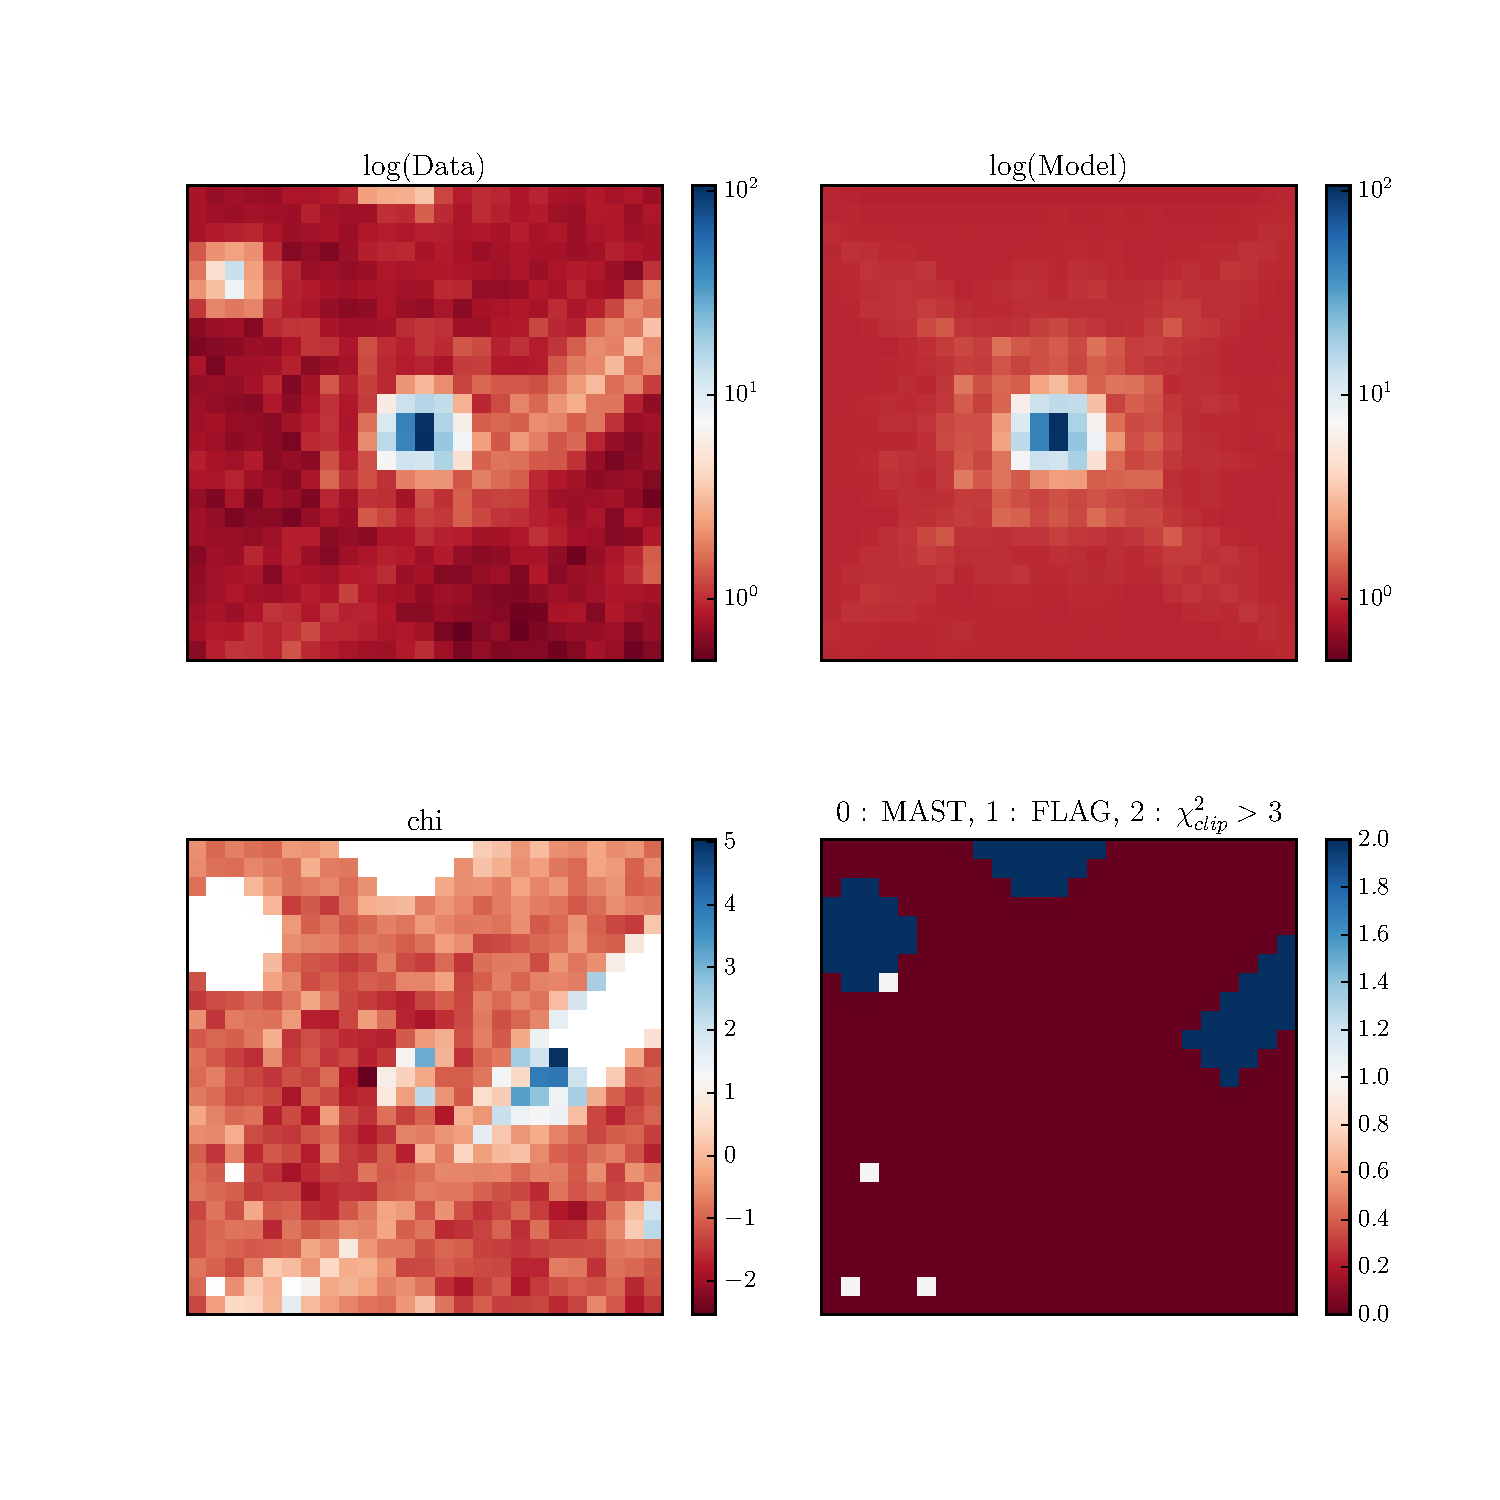
\includegraphics[width=0.9\textwidth]{figures/wfc3ir/example11.pdf}
\caption{\label{fig:validation_4} Same as Figure~\ref{fig:validation_1} but showing a different patch of the sky and and a PSF diffraction spike from a nearby source whose centroid is not in the patch. The clipping algorithm masks out most of the pixels that are affected by the PSF tail from an external source. Once again, this demonstrates the need to adopt the more conservative masking algorithm that grows the clipped regions in every direction.}
\end{figure*}

\begin{figure*}
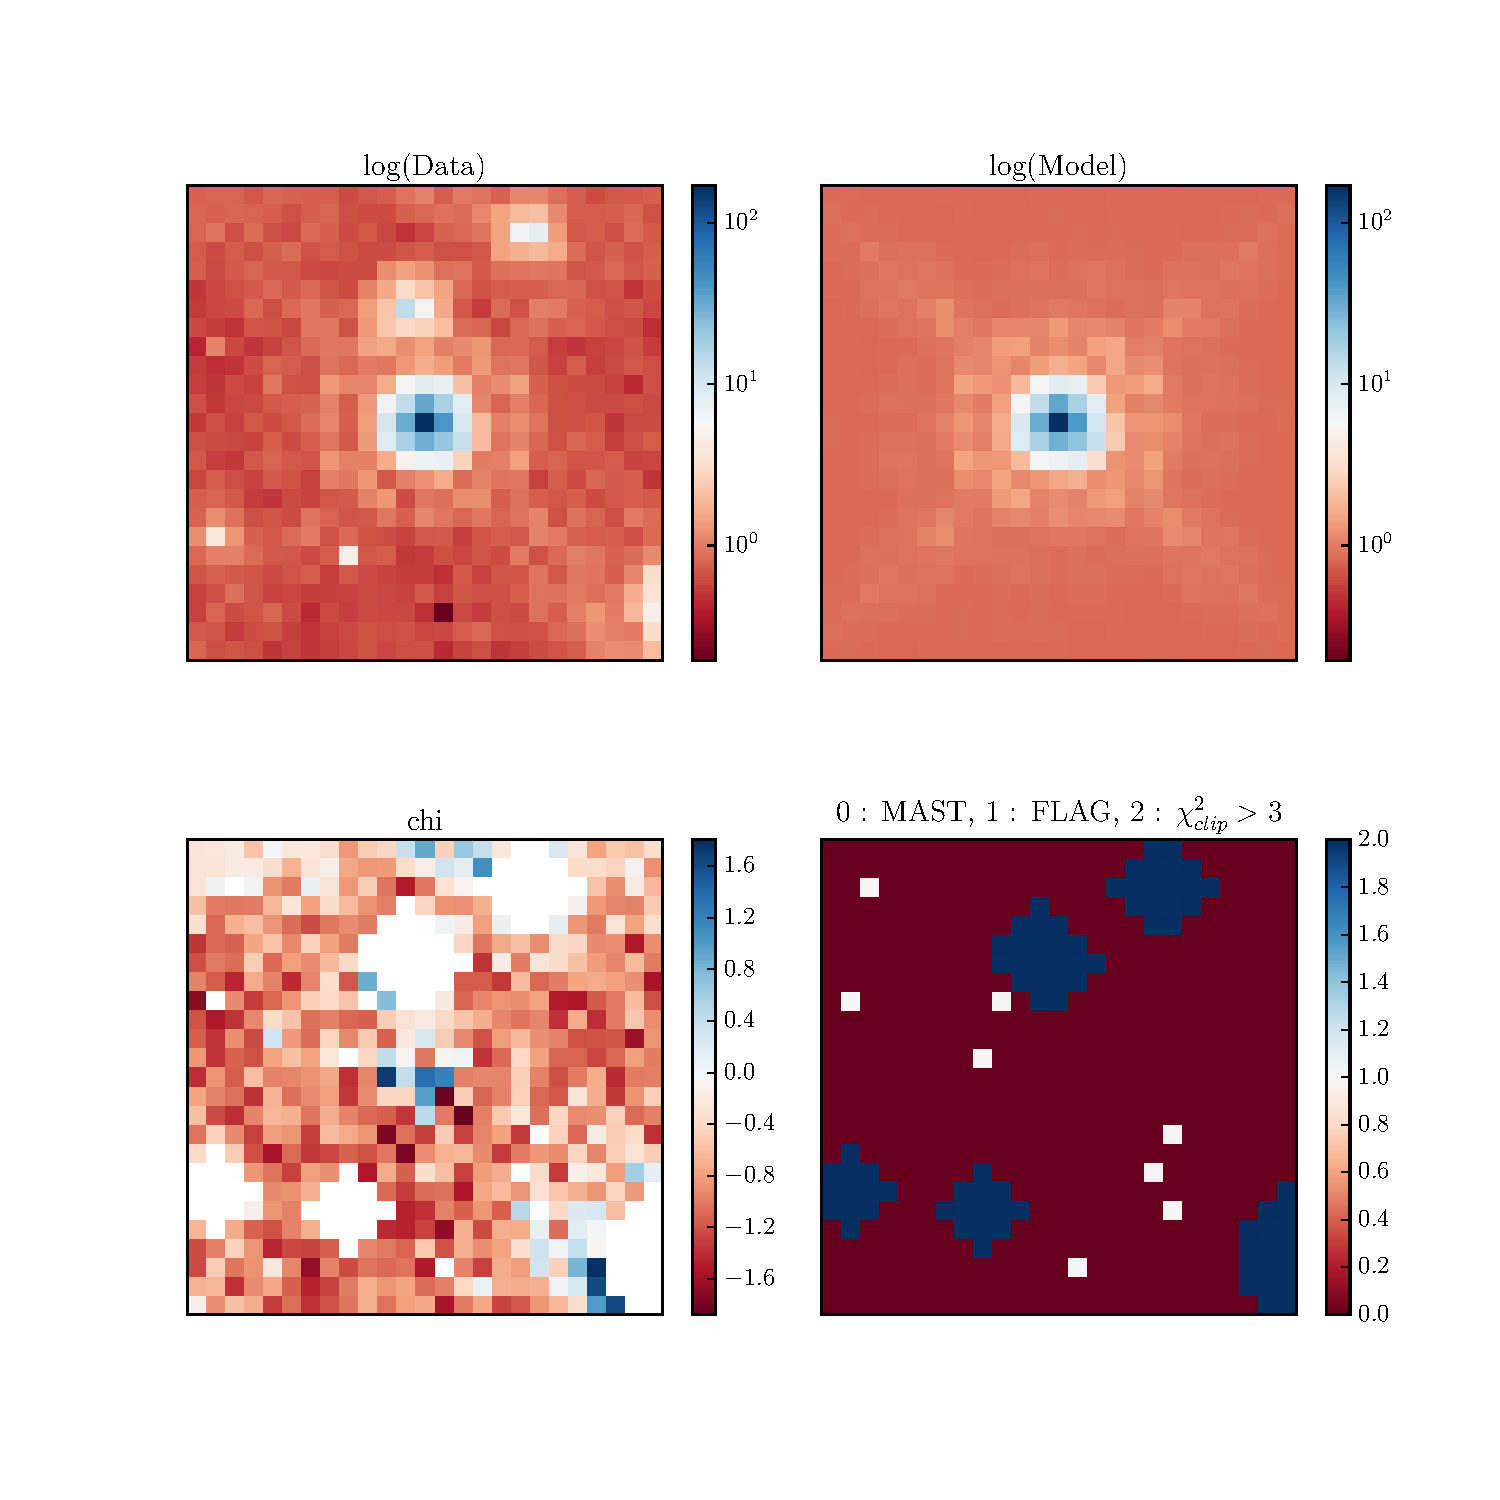
\includegraphics[width=0.9\textwidth]{figures/wfc3ir/example10.pdf}
\caption{\label{fig:validation_5} Same as Figure~\ref{fig:validation_1} but showing a different patch of sky and a more \emph{conservative} clipping algorithm. Masked regions containing the pixels with $\chi^{2}_{\rm clip} > 3$ are grown in every direction with one pixel.}
\end{figure*}

\begin{figure*}
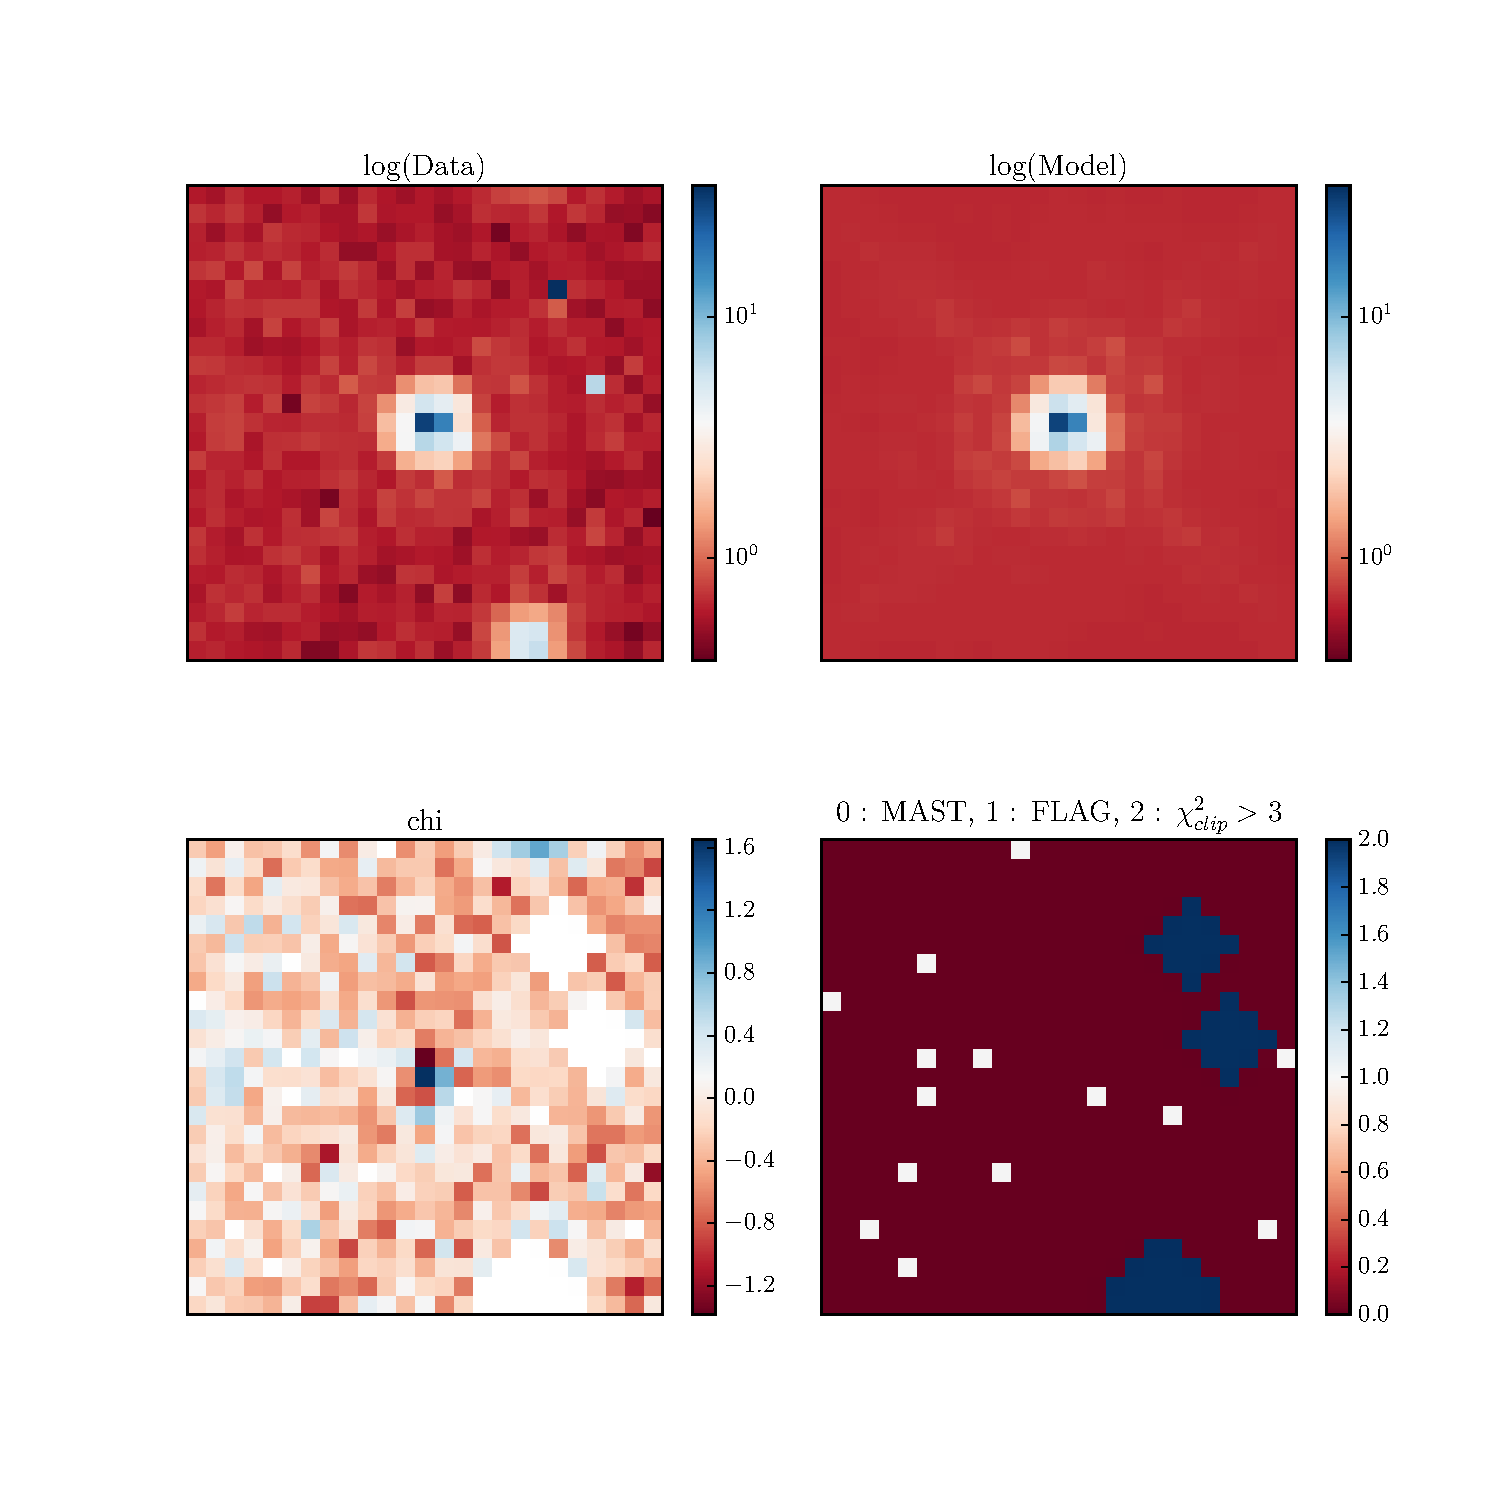
\includegraphics[width=0.9\textwidth]{figures/wfc3ir/example16.pdf}
\caption{\label{fig:validation_6} Same as Figure~\ref{fig:validation_5} but showing a different patch of sky. The more \emph{conservative} clipping algorithm masks out pixels that are ill-fit given the downsampled PSF model given by Eq.~\ref{eq:model}.}
\end{figure*}

\begin{figure*}
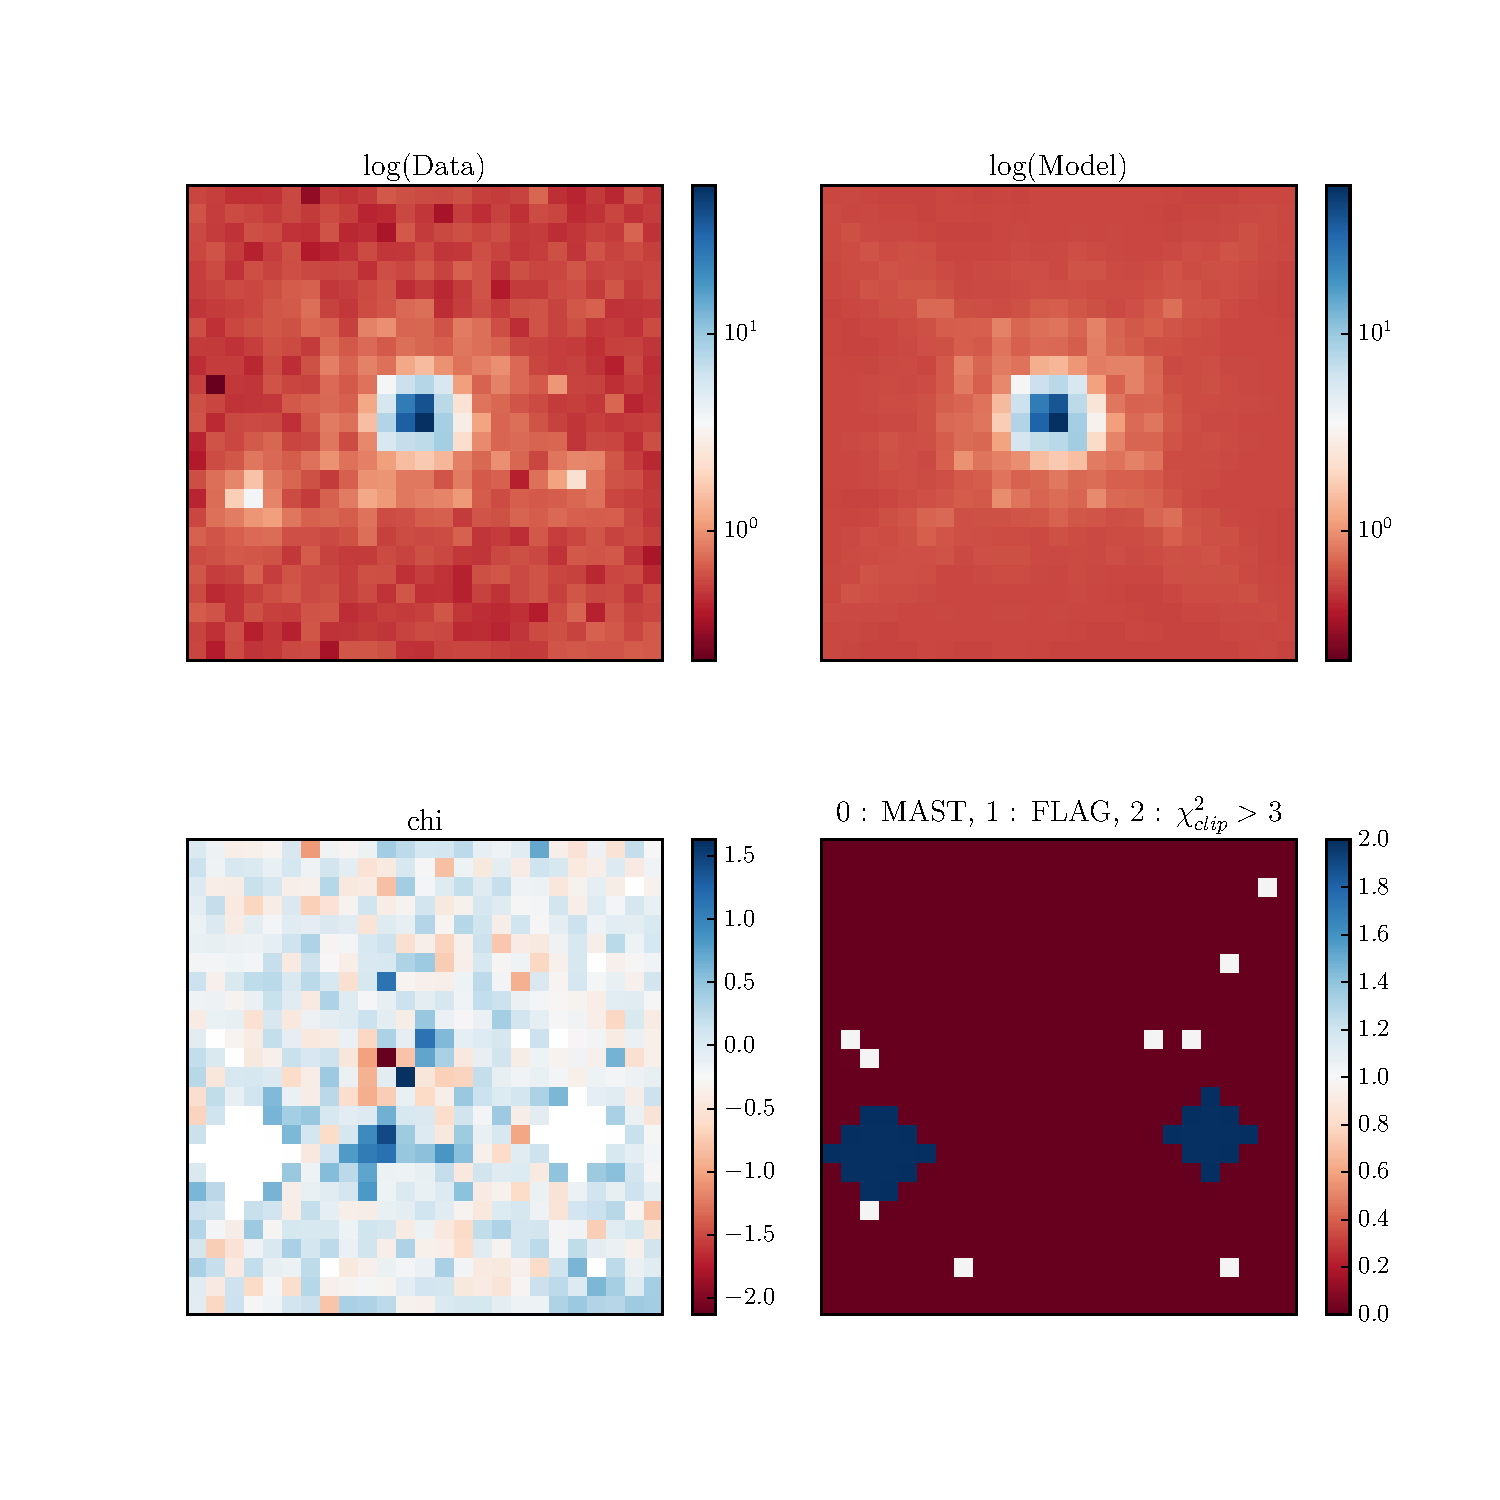
\includegraphics[width=0.9\textwidth]{figures/wfc3ir/example19.pdf}
\caption{\label{fig:validation_7} Same as Figure~\ref{fig:validation_5} but showing a different patch of sky. Note that the pixels along the lower tails of the PSF receive light contribution from other point sources and are masked out in the $\chi$-map.}
\end{figure*}


